\documentclass[%
 reprint,
%superscriptaddress,
%groupedaddress,
%unsortedaddress,
%runinaddress,
%frontmatterverbose, 
%preprint,
%preprintnumbers,
%nofootinbib,
%nobibnotes,
%bibnotes,
 amsmath,amssymb,
 aps,
%pra,
%prb,
%rmp,
%prstab,
%prstper,
%floatfix,
]{revtex4-2}

\usepackage{graphicx}% Include figure files
\usepackage{dcolumn}% Align table columns on decimal point
\usepackage{bm}% bold math
\usepackage[english]{babel}
\usepackage[utf8]{inputenc}
\usepackage{color,colortbl,multirow}
\definecolor{Gray}{gray}{0.8}
\bibliographystyle{apsrev4-2}
\usepackage{tabularx}
\usepackage[table]{xcolor}
\definecolor{Gray}{gray}{0.9} % or just use gray!15 below and skip this line
\newcolumntype{W}[1]{>{\hsize=#1\hsize\raggedleft\arraybackslash}X} % numbers right-aligned
\newcolumntype{C}[1]{>{\hsize=#1\hsize\centering\arraybackslash}X}  % centered cells
\usepackage{caption}
%\usepackage{subcaption} 
\usepackage{array}
\usepackage{subfigure}
\usepackage{placeins}
\usepackage{float}

\usepackage{colortbl}
\usepackage{hyperref}
\hypersetup{
    colorlinks=true,
    linkcolor=blue,
    citecolor=blue,
    urlcolor=blue,
    filecolor=blue
}
\makeatletter
\restylefloat{figure}

    \def\CT@@do@color{%
      \global\let\CT@do@color\relax
            \@tempdima\wd\z@
            \advance\@tempdima\@tempdimb
            \advance\@tempdima\@tempdimc
    \advance\@tempdimb\tabcolsep
    \advance\@tempdimc\tabcolsep
    \advance\@tempdima2\tabcolsep
            \kern-\@tempdimb
            \leaders\vrule
    %^^A                     \@height\p@\@depth\p@
                    \hskip\@tempdima\@plus  1fill
            \kern-\@tempdimc
            \hskip-\wd\z@ \@plus -1fill }
    \makeatother








\begin{document}


\title{Classification of transient object light curves\\using LSTM neural networks}% Force line breaks with \\

\author{Guilherme Grancho D. Fernandes$^{1,3}$, Marco Antônio Barroca$^{1}$, Mateus dos Santos$^{1}$, Rafael Santos Oliveira$^{2}$}

\affiliation{$^{1}$Centro Brasileiro de Pesquisas Físicas,\\ $^{2}$Universidade Federal de Minas Gerais,\\ $^{3}$Instituto Superior Técnico}


\date{\today}

\begin{abstract}
One of the main applications of artificial intelligence (AI) in the scientific area is as a classifier for experiments that have a high amount of data and require agility in analysis. We implemented a Long Short-Term Memory (LSTM) neural network to classify light curve data from the Large Synoptic Survey Telescope (LSST) experiment as part of The Photometric LSST Astronomical Time-series Classification Challenge (PLAsTiCC). The original dataset contained fourteen object classes, which were reorganized into five generalized categories due to class imbalance. After preprocessing the data, including padding, temporal rescaling, and flux normalization, we trained a bidirectional LSTM network with masking layers to handle variable-length sequences. Our model achieved excellent performance for S-Like and Periodic classes, with area under the ROC curve values of 0.95 and 0.99, respectively, and area under the Precision-Recall curve values of 0.98 and 0.89. However, the model struggled with Fast and Long classes and had difficulty distinguishing between Periodic and Non-Periodic objects. When evaluated on partial light curve data (5, 10, and 20 days ahead), the model's performance degraded significantly, primarily misclassifying objects as S-Like. These results suggest that class balancing and improved preprocessing strategies, such as focusing on detection moments, could enhance the model's classification capabilities.
\end{abstract}


\maketitle



\section{Introduction}
Artificial intelligence (AI) can be classified as a research area that 
investigates ways to enable computers to perform tasks in which, until now, 
humans have better performance. AI can manifest itself in various forms, in chatbots that can understand customer problems more quickly and provide more efficient responses, in intelligent assistants that need to analyze critical information from large free-text datasets, and in scientific applications, such as classifying and making decisions on the exponentially growing astronomical data.\cite{Djorgovski_2022}

Recently, the Large Synoptic Survey Telescope (LSST) proposed a challenge on the Kaggle website, a Google subsidiary, called The Photometric LSST Astronomical Time-series Classification Challenge (PLAsTiCC).\cite{kaggle} This is a challenge aimed at classifying light curves, data of the observed brightness of celestial objects as a function of time, which were simulated in preparation for LSST observations. These curves are capable of revealing the presence of some phenomena, such as supernovae\cite{Russel_1912}. The LSST will revolutionize our understanding of the sky, however this type of study is hindered by the large volume of data obtained by the telescope, making automatic analysis procedures indispensable to differentiate and classify them. In this challenge, the question was raised: How well can we classify objects in the sky that vary in brightness from simulated LSST time-series data? From this, the need arose for a data challenge to help classify these astronomical sources and describe the PLAsTiCC dataset and the Kaggle data challenge. \cite{PLAsTiCC}



Before the use of AI, this type of classification still depended on manual analysis. Common statistical methods such as template fitting\cite{Tanvir_2005} were used, but these are not scalable for a large volume of data. Usually, a group of experts manually eliminated obvious cases of false positives, something that by itself can take several days. Of the remaining data, each case should be reviewed by at least three experts, which can lead to disagreements about a particular case, since experts might not have the same definition for classification. For these reasons, a reliable system is necessary that repeatedly selects the most important candidates that will be manually reviewed for confirmation at a later stage.




Since light curves are a function that varies with time, one of the possible ways to solve the PLAsTiCC problem is to use a Long Short-Term Memory (LSTM) Neural Network. The LSTM is a recurrent neural network (RNN) architecture, developed by Hochreiter and Schmidhuber in 1997. Recurrent networks have the characteristic of making some information persist in the network through a loop at arbitrary intervals. The RNN by definition has a simpler repetition structure than LSTMs, as there is only a single tanh layer, figure \ref{fig:RNN}, while LSTMs have a chain structure that contains four neural network layers and different memory blocks called cells as shown in figure \ref{fig:lstm}. Thus, LSTMs are well suited for classifying, processing, and predicting time series with time intervals of unknown duration. \cite{Gabriel_2022}


\begin{figure}[!ht]
    \centering
    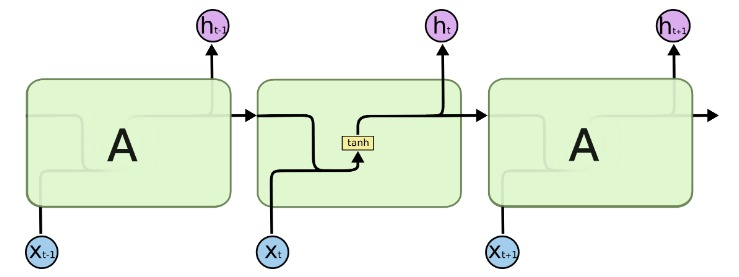
\includegraphics[width=9.0cm]{figures/RNN.jpeg}
        \caption{Functioning of an RNN network. \cite{colah}}
    \label{fig:RNN}
\end{figure}


\begin{figure}[!ht]
    \centering
    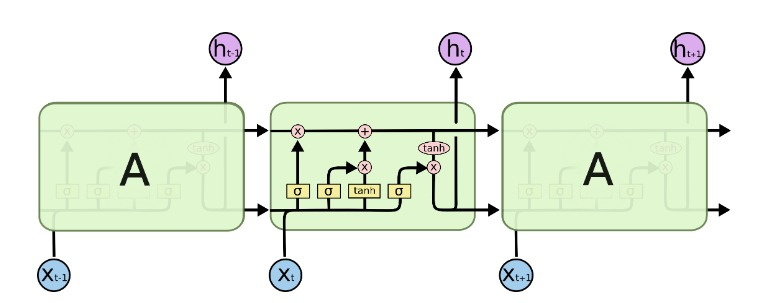
\includegraphics[width=9.0cm]{figures/LSTM.jpeg}
    \caption{Functioning of an LSTM network. \cite{colah}}
    \label{fig:lstm}
\end{figure}




\section{Methodology}

The light curve data were obtained through LSST PLAsTiCC via the Kaggle challenge\cite{kaggle}. In order to complete the project within the scheduled time of EAFEXP, a subset of the total data was used. In total, two datasets were used: the first had 7848 objects, of which 10$\%$ were used to form a validation set and the remainder formed the training set; the second dataset had 19920 objects and was used as the test set.

The data are tabular and consist of flux measurement information, measurement error, the measurement time in Modified Julian Date (mjd), the filter used (the object's emission spectrum, ugriZY, represented by a numerical value from zero to five), a boolean variable (0 or 1) that indicates detection or non-detection, the object class, and a unique identifier. An example can be seen in Table \ref{tab:conjunto-dados-ex}.

\begin{table}[ht]
\centering
\setlength{\tabcolsep}{4pt}     % less space between columns
\renewcommand{\arraystretch}{1.1}
\footnotesize                   % smaller text (optional)
\resizebox{\columnwidth}{!}{%   % ensures it fits in the column
\begin{tabular}{|r|r|r|c|c|c|r|}
\hline
\textbf{Flux} & \textbf{Error} & \textbf{mjd} & \textbf{Filter} & \textbf{Detection} & \textbf{Class} & \textbf{Id} \\\hline
-544.810 & 3.623  & 59750.4 & 2 & 1 & 92 & 615 \\\hline
-816.434 & 5.553  & 59750.4 & 1 & 1 & 88 & 713 \\\hline
-471.386 & 3.802  & 59750.4 & 3 & 1 & 42 & 730 \\\hline
... & ... & ... & ... & ... & ... & ... \\\hline
-388.985 & 11.395 & 59750.4 & 4 & 1 & 90 & 745 \\\hline
-2.940   & 1.771  & 59798.3 & 3 & 0 & 90 & 116720 \\\hline
-12.810  & 5.380  & 59798.4 & 5 & 0 & 92 & 117016 \\\hline
... & ... & ... & ... & ... & ... & ... \\\hline
\end{tabular}}
\caption{Table exemplifying the dataset.}
\label{tab:conjunto-dados-ex}
\end{table}






\subsection{Preprocessing}

Initially, the provided data had fourteen categories, however due to the discrepancy in the amount of data per category, the data were reorganized into five categories according to Table \ref{tab:classes-generalizadas}. Examples of each of the classes can be seen in figure \ref{fig:curvas}. The distribution by original classes and generalized classes can be seen in figure \ref{fig:classes}.


\begin{table}[ht]
\centering
\setlength{\tabcolsep}{4pt}
\renewcommand{\arraystretch}{1.1}
\footnotesize
\resizebox{\columnwidth}{!}{%
\begin{tabular}{|r|l|l|r|}
\hline
\rowcolor{gray!20}\textbf{Id} & \textbf{Original Class} & \textbf{Generalized Class} & \textbf{New Id} \\\hline
6  & Single micro-lens & Fast         & 1 \\\hline
15 & TDE               & Long         & 2 \\\hline
16 & Eclipsing Binary  & Periodic     & 3 \\\hline
42 & SNII              & S-Like       & 0 \\\hline
52 & SNIax             & S-Like       & 0 \\\hline
53 & Mira              & Periodic     & 3 \\\hline
62 & SNIbc             & S-Like       & 0 \\\hline
64 & Kilonova          & Fast         & 1 \\\hline
65 & M-dwarf           & Fast         & 1 \\\hline
67 & SNIa-91bg         & S-Like       & 0 \\\hline
88 & AGN               & Non-Periodic & 4 \\\hline
90 & SNIa              & S-Like       & 0 \\\hline
92 & RR lyrae          & Periodic     & 3 \\\hline
95 & SLSN-I            & Long         & 2 \\\hline
\end{tabular}}
\caption{Table with the fourteen original classes and their generalized classes.}
\label{tab:classes-generalizadas}
\end{table}



\begin{figure}[]
    \centering
    \subfigure[Distribution of measurements by original classes.]{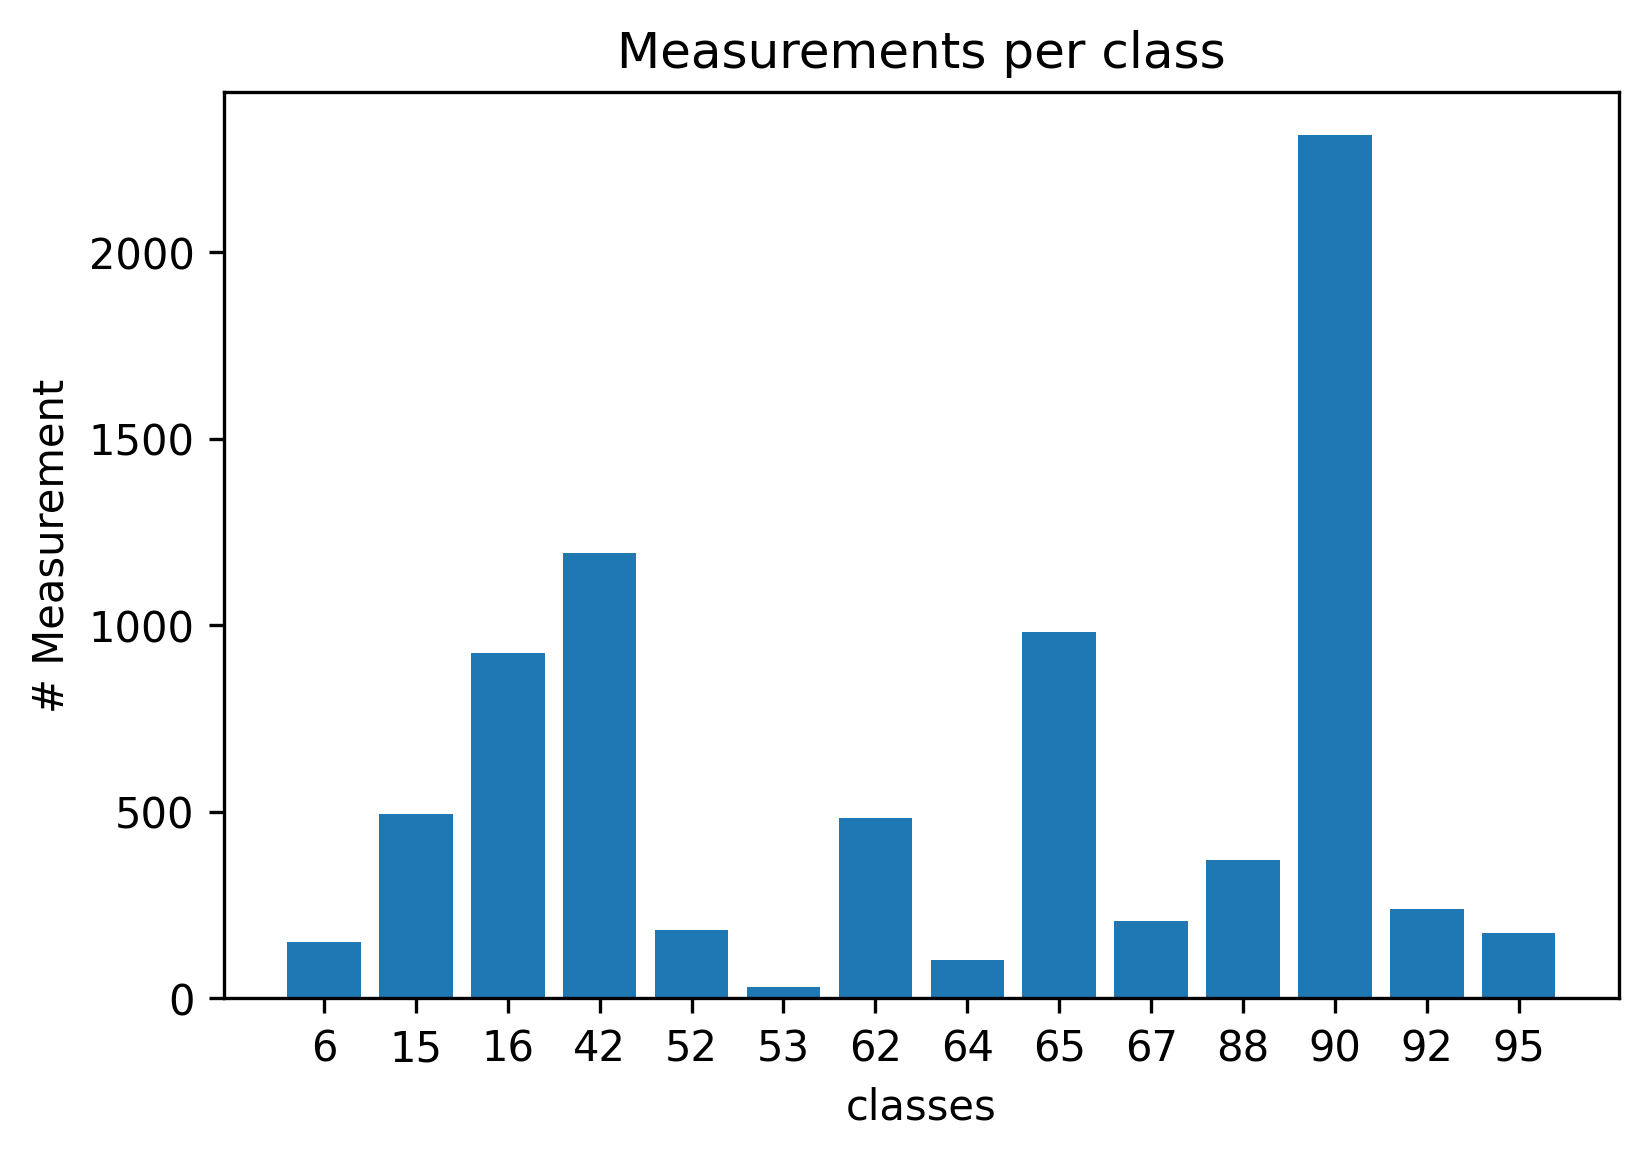
\includegraphics[width=6.7cm]{figures/14_classes_new.png}}
    \hfill
    \subfigure[Distribution of measurements by generalized classes.]{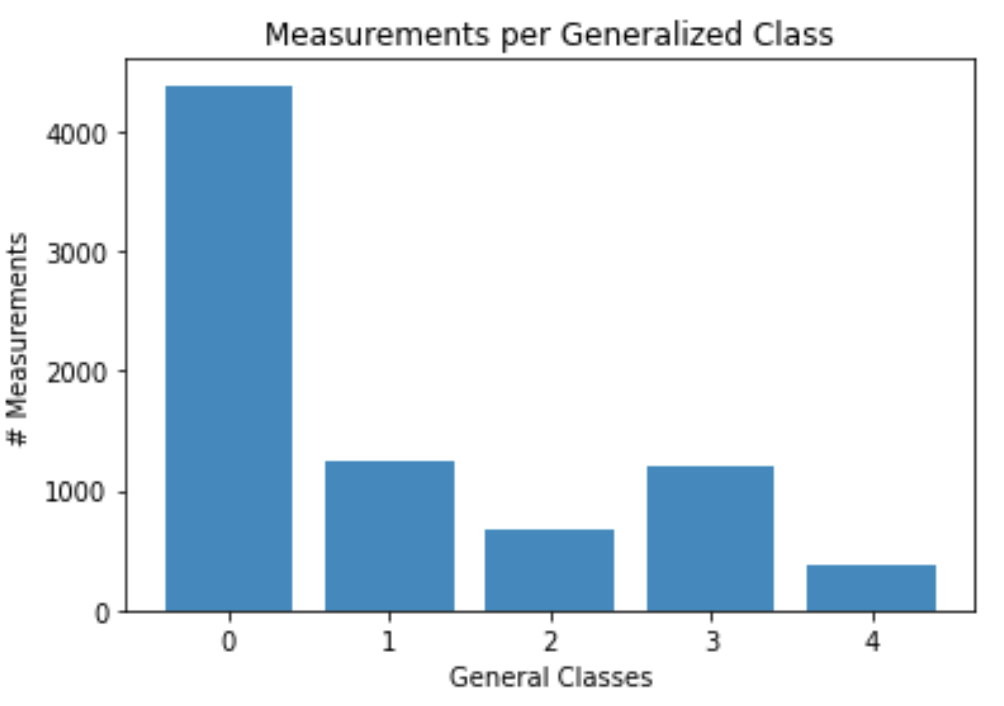
\includegraphics[width=6.7cm]{figures/fig_1.png}}
    \caption{}
    \label{fig:classes}
\end{figure}
\newpage

To train the network, it is necessary to ensure that each object has the same number of measurements, since this will be the input dimension. This is not true for this dataset, so the data with smaller dimensions were filled with arbitrary values in a process known as padding. It can be observed in figure \ref{fig:padding} that after padding, all objects have the same dimension.

In addition, the temporal measurements were rescaled so that the first measurement of an object was considered as zero on the temporal scale, and finally, the flux data needed to be normalized for each object separately since the amplitude of measurements between objects is not constant.

Finally, this project is interested in verifying the ability to classify objects with only partial light curve data. For this purpose, two new test sets were selected, where the data were advanced in time by ten and twenty days of observation from the moment each object is detected, and subsequently the network was evaluated with sets of five, ten, and twenty days into the future.

\begin{figure}[!h]
    \centering
    \subfigure[Distribution of the number of measurements per object.]{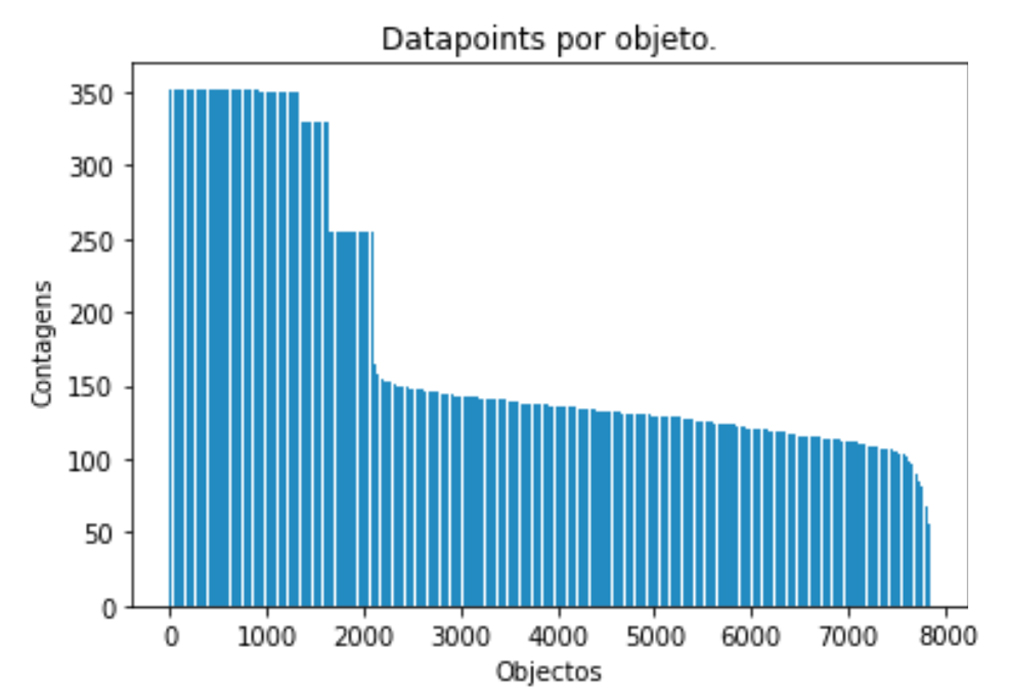
\includegraphics[width=.49\textwidth]{figures/fig_42.jpg}}
    \hfill
    \subfigure[Distribution of the number of measurements per object after padding.]{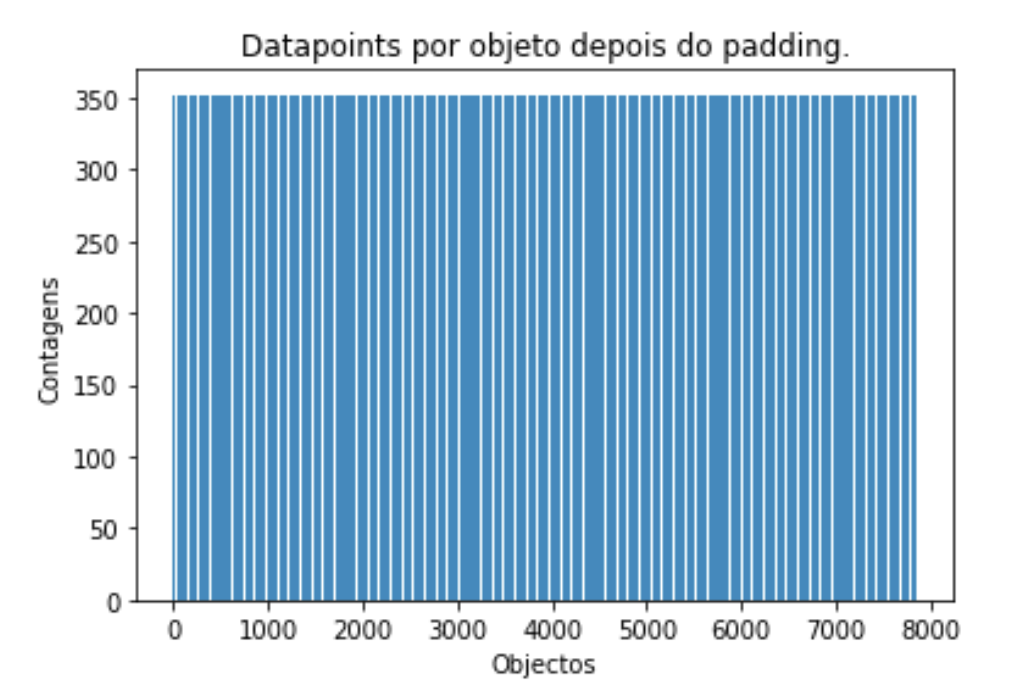
\includegraphics[width=.49\textwidth]{figures/fig_4.png}}
    \caption{}
    \label{fig:padding}
\end{figure}
\newpage

\subsection{Neural Network}

Since the provided data are time series, the use of an LSTM network was chosen. The network will be bidirectional because previous measurements are as relevant as subsequent measurements. It was also decided that each of the columns in the dataset exemplified in table \ref{tab:conjunto-dados-ex} will be treated as a feature of the object.

Due to the padding procedure, all objects came to have 352 measurements and 5 features. This means that the input dimensions of the network will be 352x5 and the output will be a probability distribution in a tensor of size five, since we have 5 generalized classes.

Due to the padding performed, it is necessary to have a mask layer so that the arbitrary data are identified and ignored by the network. Otherwise, they would be treated as noise in the dataset.

It will also be necessary to use a dense layer to perform the classification process and a GlobalMaxPooling layer to reduce the dimensions of the problem. The complete network can be visualized in figure \ref{fig:rede}.

\begin{figure*}[]
    \centering
    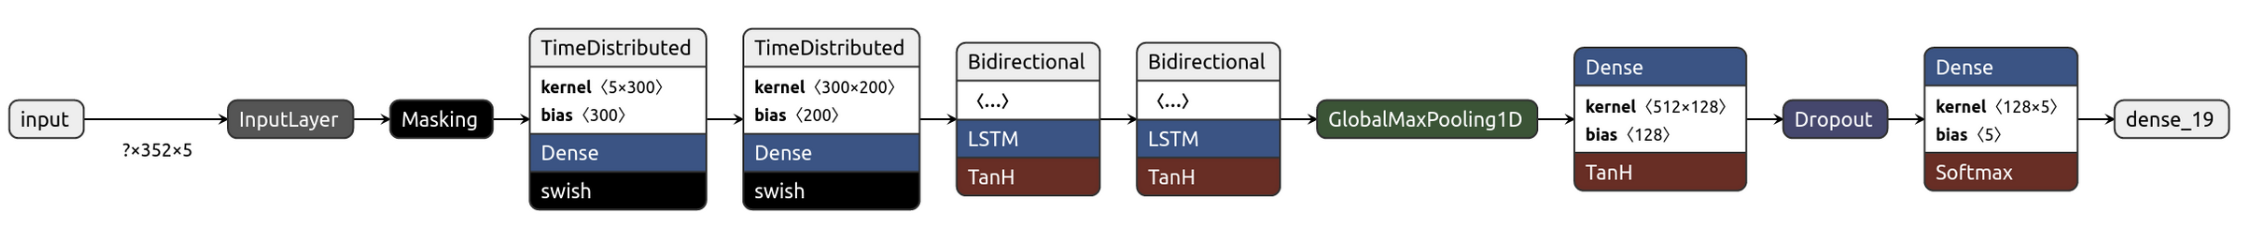
\includegraphics[width=\textwidth]{figures/rede.png}
    \caption{Neural network used in the classification process. The LSTM network is bidirectional because equal importance must be given to past and future data; the Mask layer serves to attenuate the noise effects that padding can cause}
    \label{fig:rede}
\end{figure*}


\section{Results and Discussion}

The metrics chosen for network evaluation were ROC curves, Precision-Recall curves, and a confusion matrix. The network's performance with partial light curve data was also verified. All these metrics were constructed using the test set.

The ROC curves obtained were mostly excellent, achieving area under the curve values for the S-Like and Periodic classes of 0.95 and 0.99, respectively. The same cannot be said for the Long class, for which a value of 0.68 was obtained. 

Similarly, the values achieved for the Precision-Recall curves for the S-Like and Periodic classes obtained high area under the curve values, 0.98 and 0.89, respectively. For the Non-Periodic class, the worst result of 0.40 was obtained. All curves can be visualized in figure \ref{fig:RoC_Recall}.

By observing the confusion matrix, it is easier to understand what is happening. The classification of S-Like curves is done with high accuracy, and the model is still capable of distinguishing curves from the Periodic and Non-Periodic classes from the other three. However, it can be seen that the model completely fails when trying to classify Long or Fast type curves and is also unable to differentiate Periodic and Non-Periodic curves from each other. The matrix can be visualized in figure \ref{fig:matrizes} (a).

\begin{figure}[]
    \centering
    \subfigure[ROC curve for our classification model. The Periodic and S-Like classes show satisfactory results, however the same cannot be said for the Fast and Long classes.]{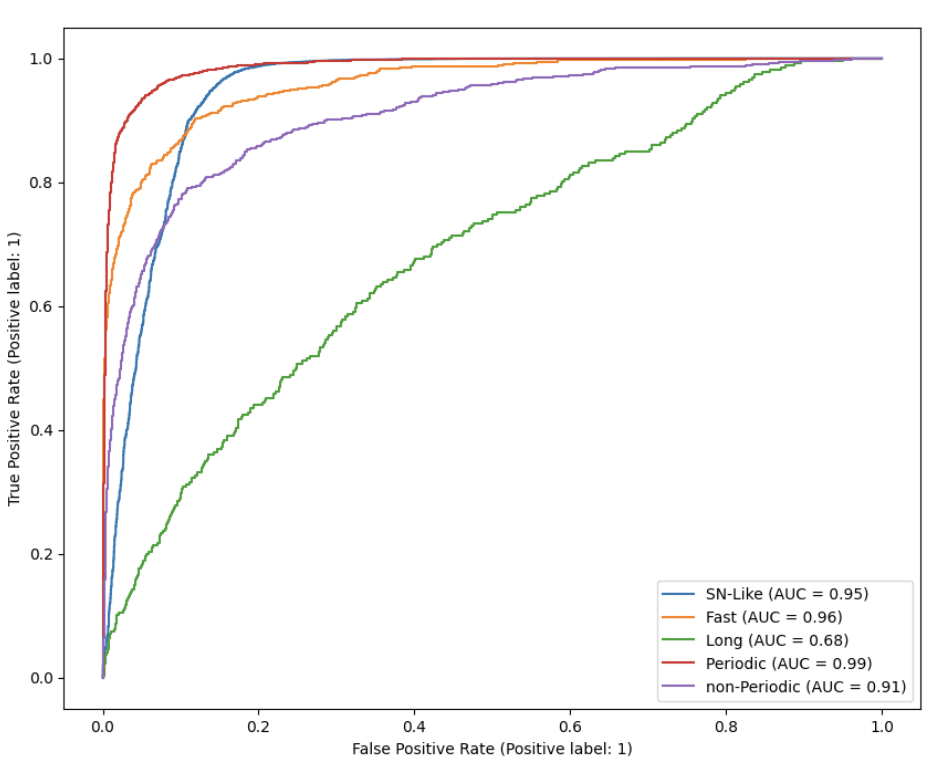
\includegraphics[width=6.7cm]{figures/RoC.png}}
    \hfill
    \subfigure[Precision-Recall curve for our classification model. The Periodic and S-Like classes show satisfactory results, however we notice that the model does not seem to correctly classify Non-Periodic curves. ]{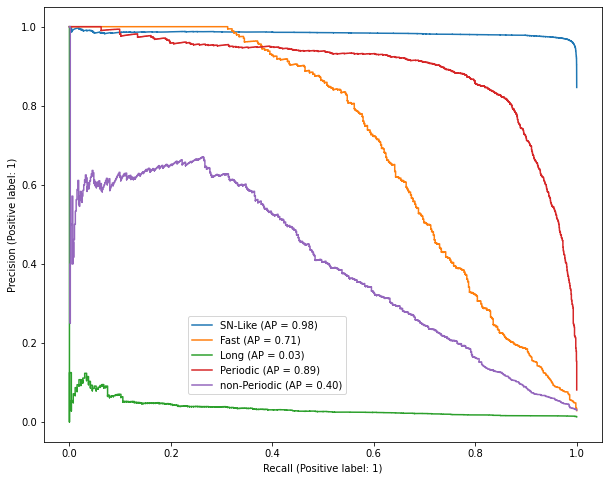
\includegraphics[width=6.7cm]{figures/Pre_Rec.png}}
    \caption{}
    \label{fig:RoC_Recall}
\end{figure}


As mentioned earlier, it is necessary to evaluate the network on 
test sets that were advanced in time; in this case, it was evaluated at five, ten, and twenty days. Thus, it is possible to see that the confusion matrix shows worse results as the test set is advanced in time, and even with five days of advance, the network is unable to classify objects with performance similar to the complete set and begins to confuse all objects with the S-Like class. In figure \ref{fig:matrizes} (b), (c), and (d), the confusion matrices for the different test sets are shown.

\begin{figure*}[!h]
    \centering
    \subfigure[Confusion matrix for the complete test set.]{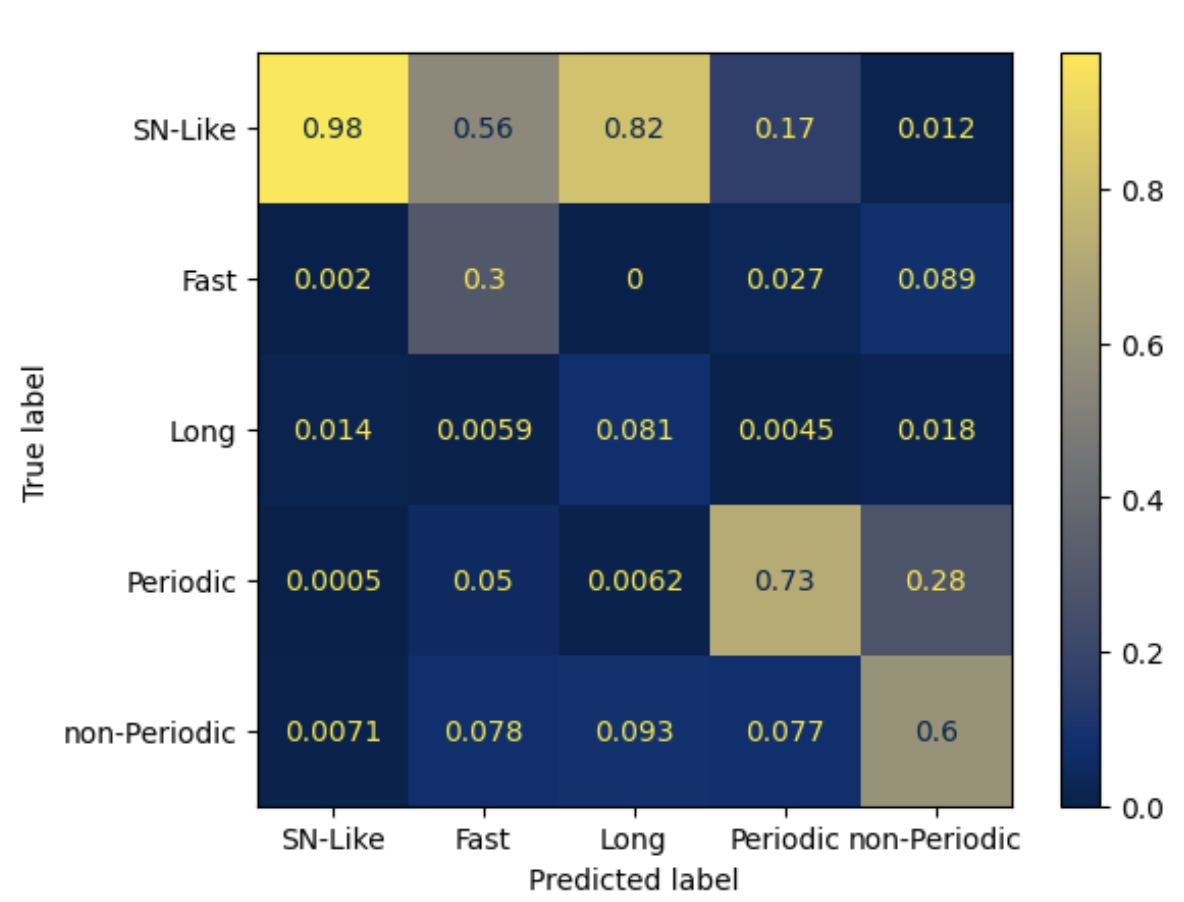
\includegraphics[width=\columnwidth]{figures/matriz.png}}
    \hfill
    \subfigure[Confusion matrix for the test set with five days ahead. The results worsen compared to the complete test set.]{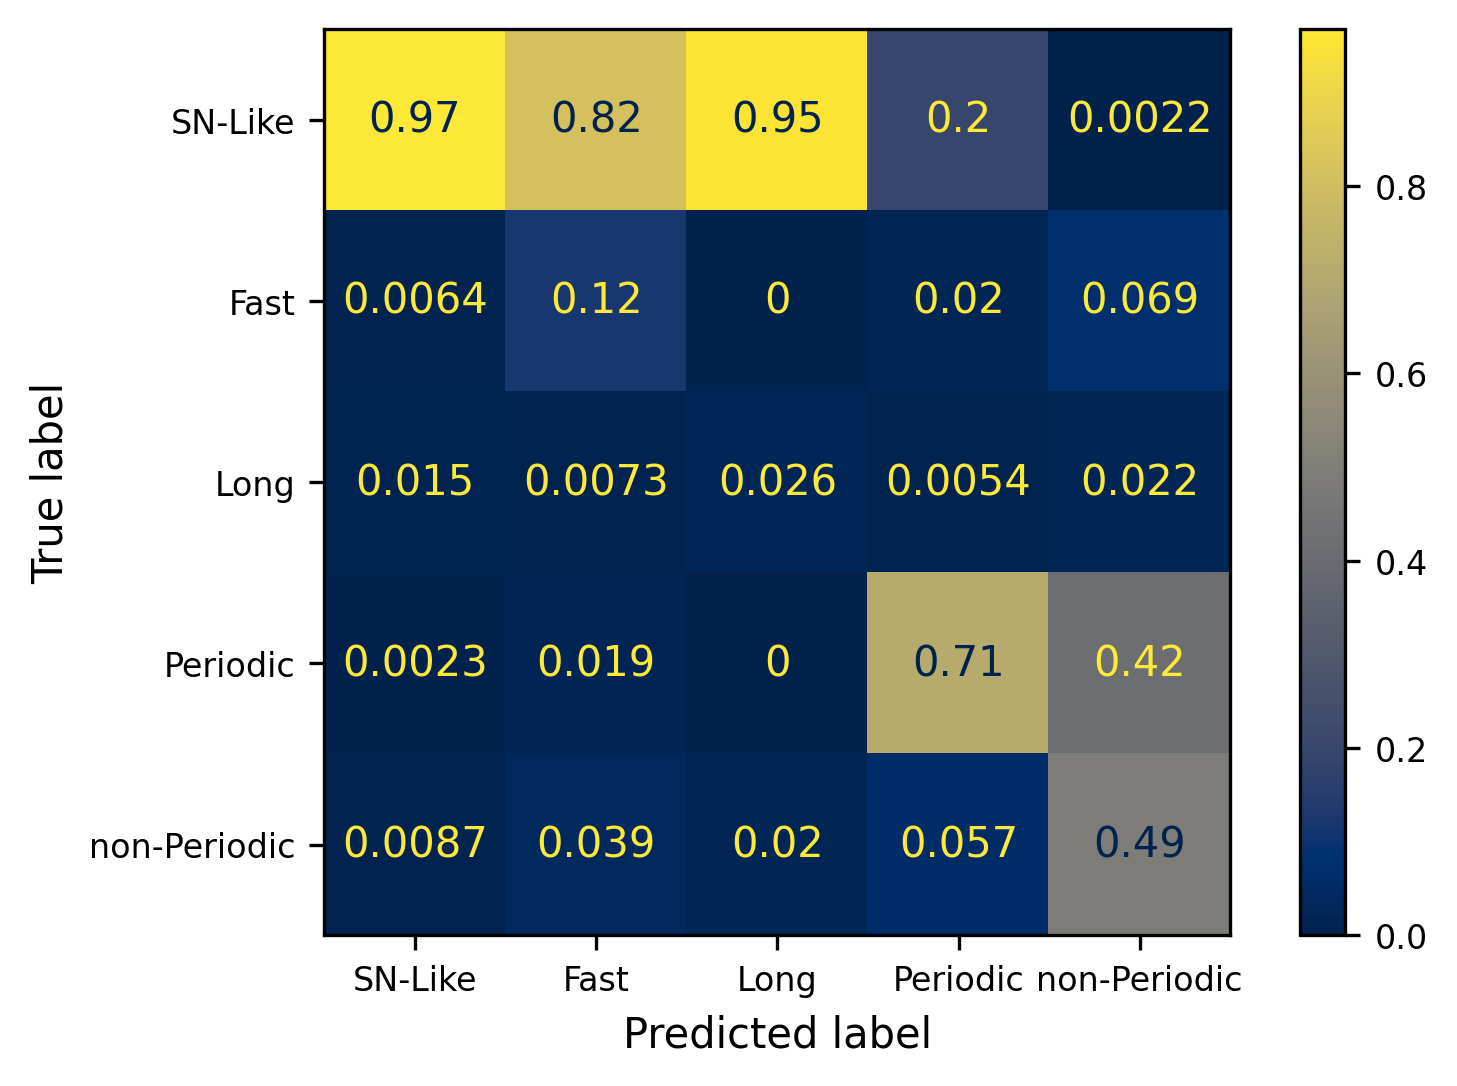
\includegraphics[width=\columnwidth]{figures/matrix_5.png}}
    \hfill
    \subfigure[Confusion matrix for the test set with data ten days ahead. The results worsen compared to the sets with ten and five days.]{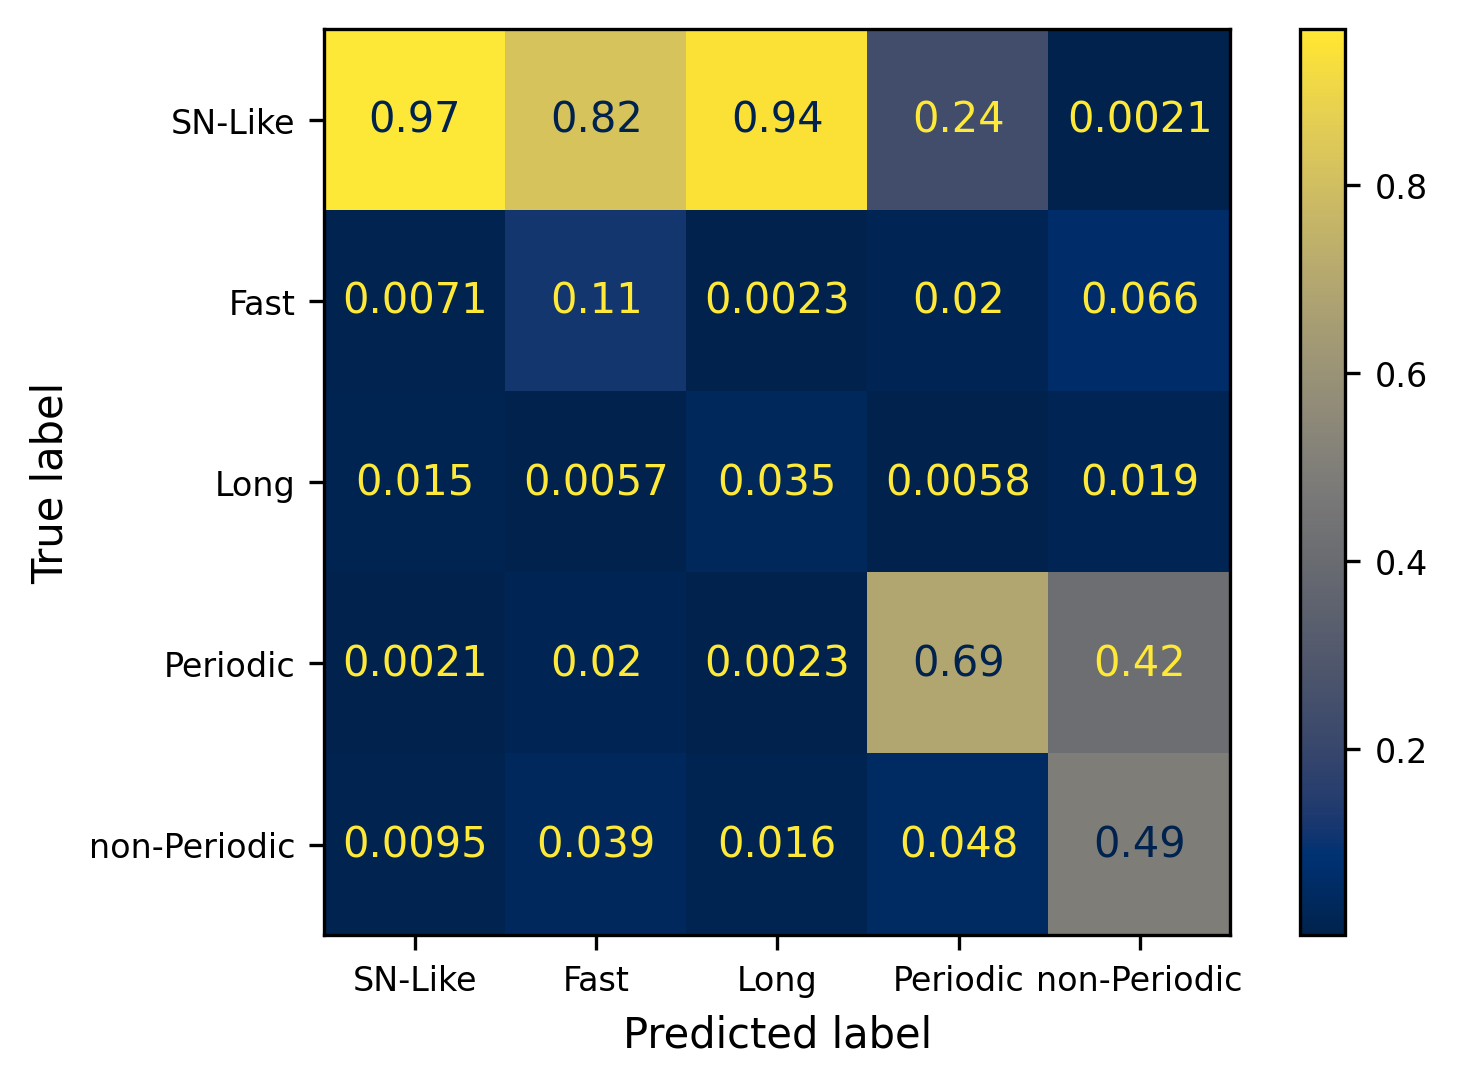
\includegraphics[width=\columnwidth]{figures/matriz_10.png}}
    \hfill
    \subfigure[Confusion matrix for the test set with data twenty days ahead. The network now confuses more classes with S-Like type objects.]{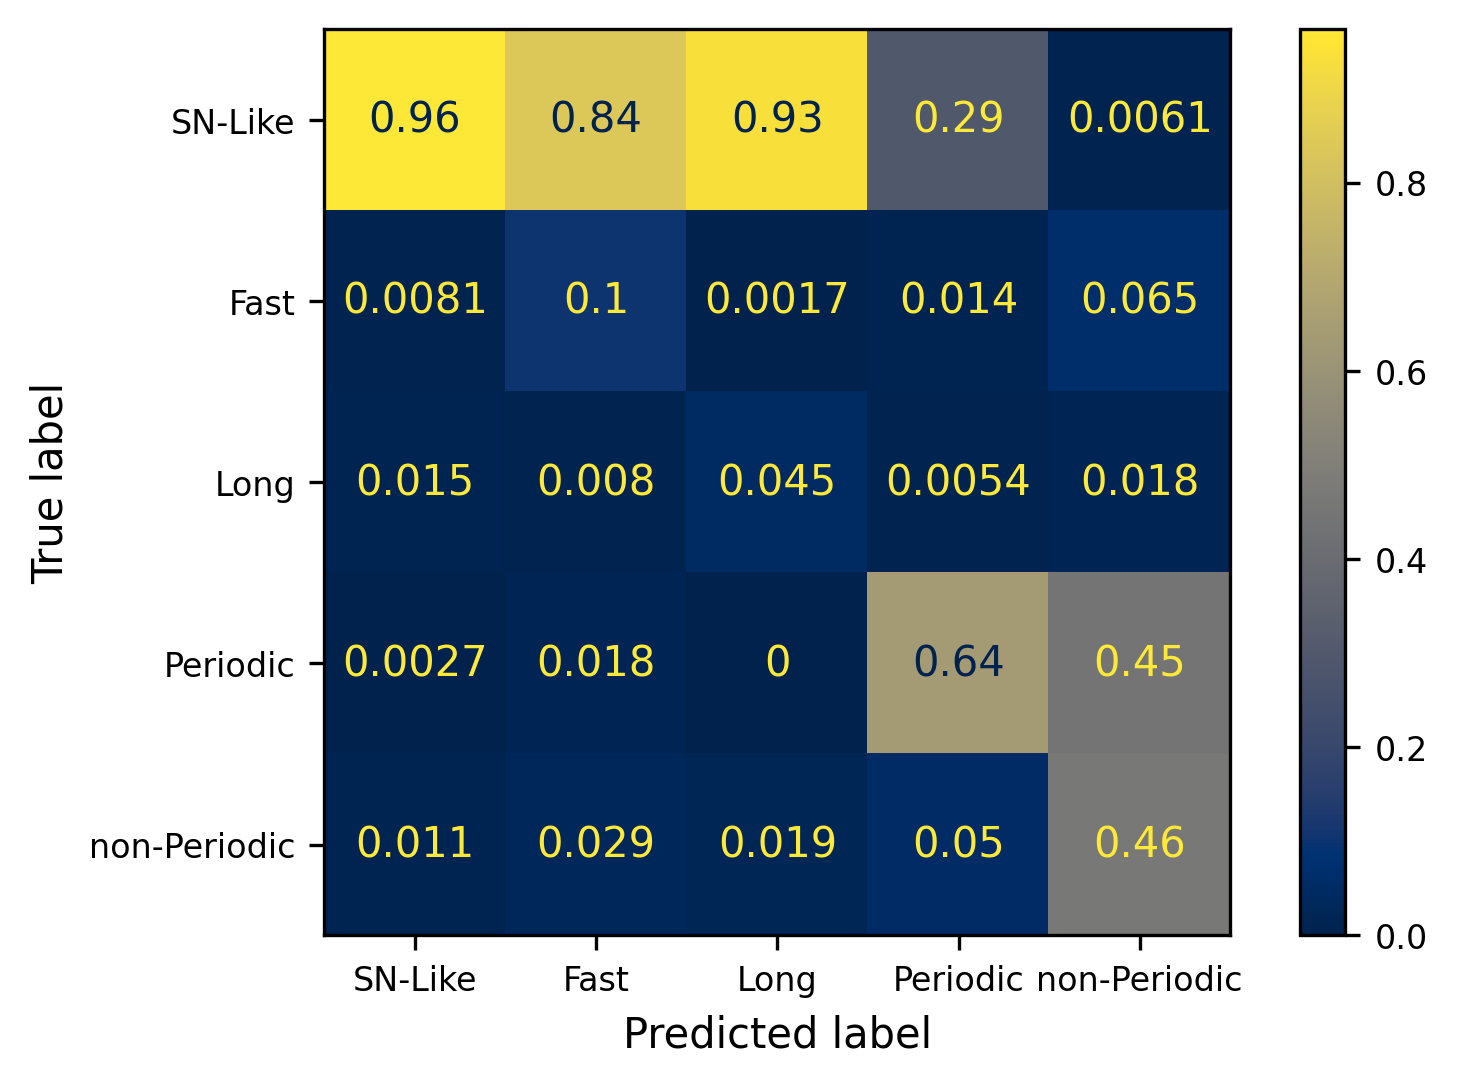
\includegraphics[width=\columnwidth]{figures/matriz_20.png}}
    \caption{}
    \label{fig:matrizes}
\end{figure*}




\section{Conclusion}

The neural network developed in this project was able to classify S-Like objects and still distinguish Periodic and Non-Periodic objects from the others. Unfortunately, these results do not repeat for the Fast and Long classes, probably due to the difficult characterization of these curves that have short-duration peaks only at the beginning or end of the measurement.

Another problem that this model presents is that it is not possible to effectively distinguish Non-Periodic objects, confusing them with Periodic objects. This result probably comes from the fact that both curves show several peaks throughout the measurement, and the model seems to attribute periodicity to measurements that are not periodic. Despite this, the network almost never identifies periodic measurements as non-periodic.

Finally, unfortunately, this network loses the ability to classify any object when partial light curve data are provided and begins to confuse all objects as if they were S-Like. This is likely due to the fact that the dataset, even with generalized classes, still shows a high prevalence of the S-Like class. The network's confusion in classifying non-periodic objects, recognizing them as periodic, is also noticeable.

As a suggestion to correct these problems, one could consider choosing a training set that is more balanced in its class distribution. Including more Non-Periodic type objects in the network training set may be sufficient to reduce confusion with the Periodic class. 


During the production of this work, one of the solutions attempted to minimize the class imbalance problem was the use of weights during network training; however, this technique did not show a significant improvement for classification.

Regarding solving the classification issue for Fast and Long objects, it may be necessary to change the data preprocessing. For example, one could extract from the data the moments when the boolean detection variable has value 1 and use only those portions of the light curves. In this way, background data from the object would be removed, keeping only the measurements corresponding to detections. This could also help with the issue of classification with partial curve data.

\begin{figure*}[]
    \centering
    \subfigure[Example of a light curve of an object from the S-Like class. The values in the legend indicate the filter used and the emission spectrum.]{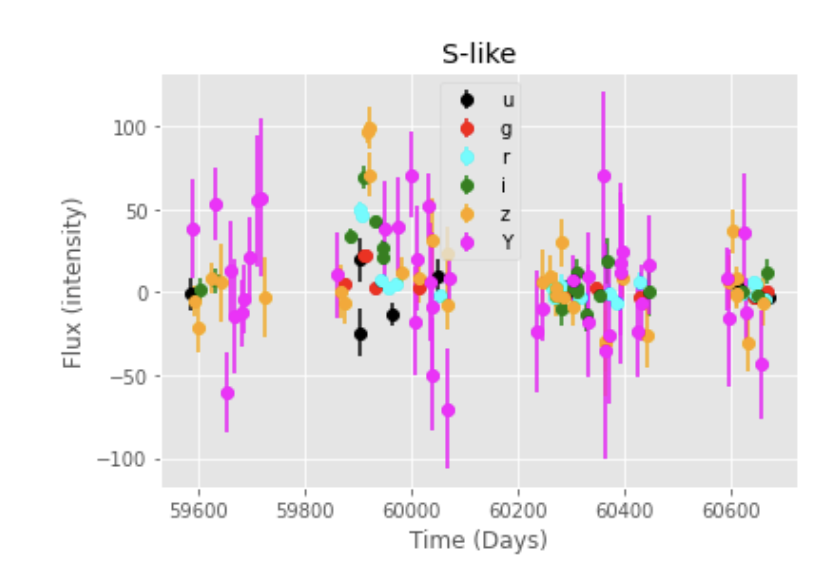
\includegraphics[width=\columnwidth]{figures/S_like_ex.png}}
    \hfill
    \subfigure[Example of a light curve of an object from the Fast class. The values in the legend indicate the filter used and the emission spectrum.]{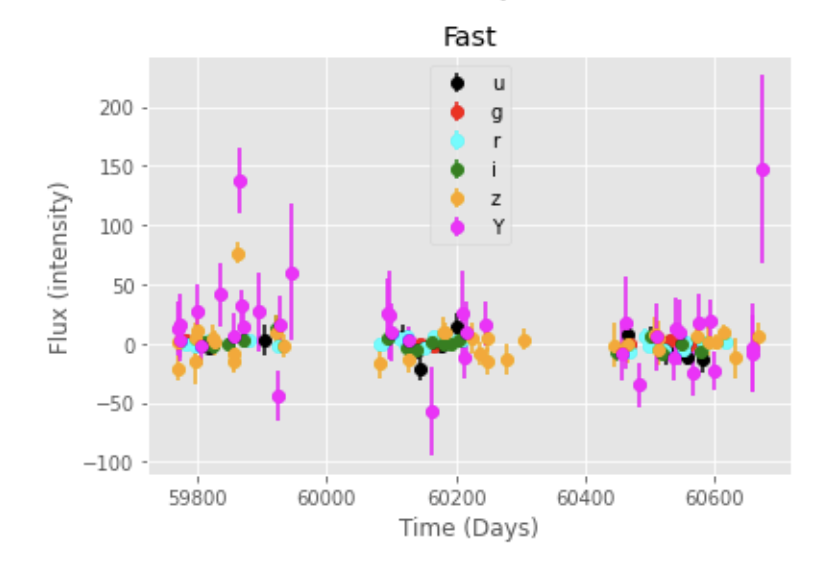
\includegraphics[width=\columnwidth]{figures/Fast_ex.png}}
    \hfill
    \subfigure[Example of a light curve of an object from the Long class. The values in the legend indicate the filter used and the emission spectrum.]{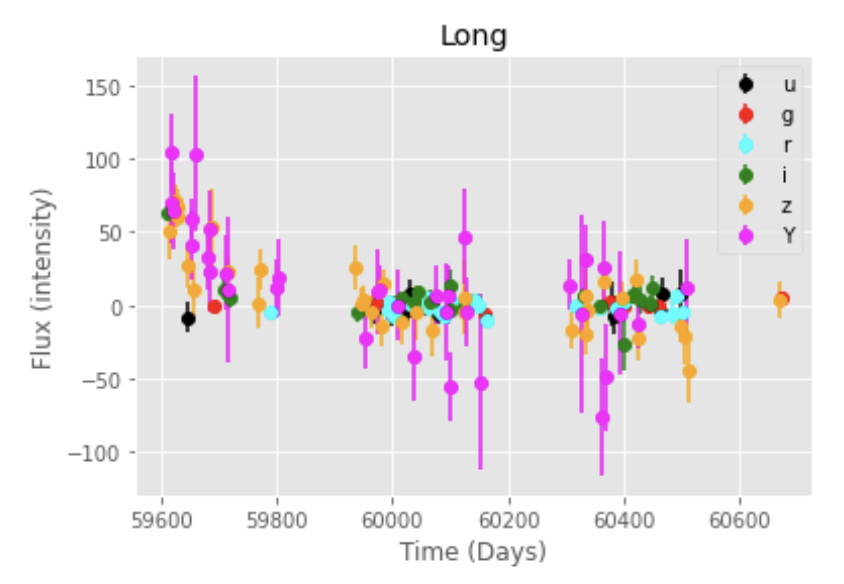
\includegraphics[width=\columnwidth]{figures/Long_ex.png}}
    \hfill
    \subfigure[Example of a light curve of an object from the Periodic class. The values in the legend indicate the filter used and the emission spectrum.]{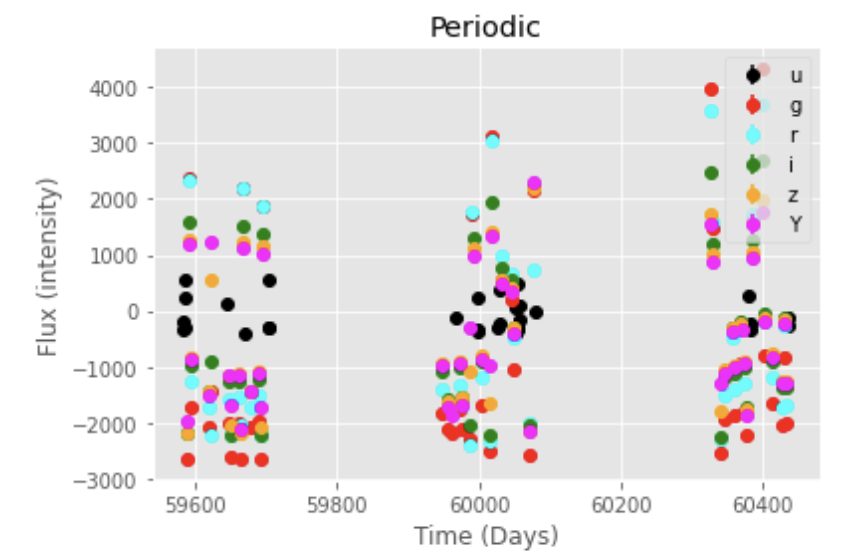
\includegraphics[width=\columnwidth]{figures/Periodic_ex.png}}
    \hfill
    \subfigure[Example of a light curve of an object from the Non-Periodic class. The values in the legend indicate the filter used and the emission spectrum.]{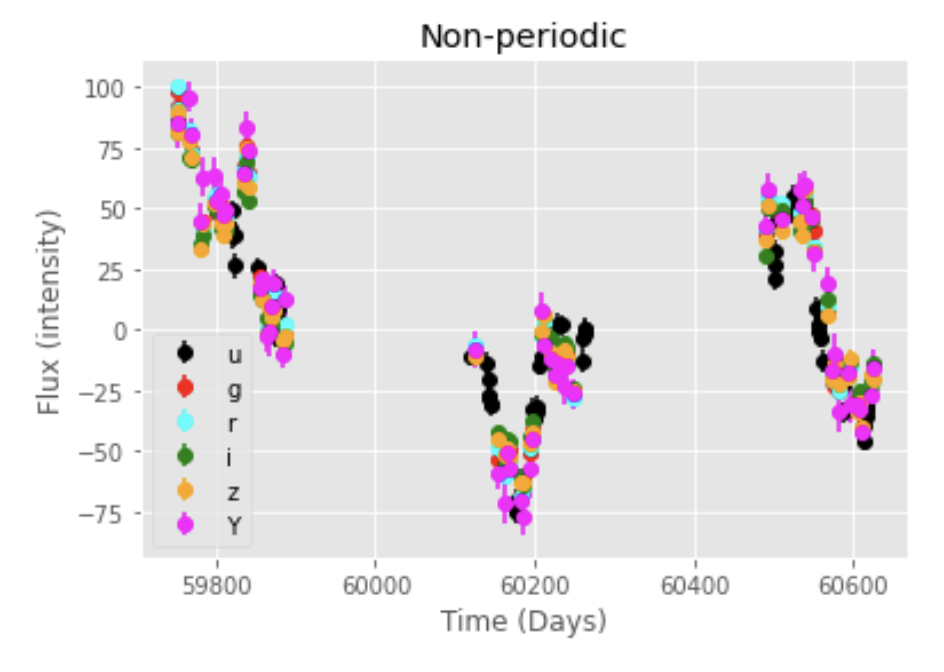
\includegraphics[width=\columnwidth]{figures/Non_periodic_ex.png}}
    \caption{}
    \label{fig:curvas}
\end{figure*}

\section{Code}

All code used and the trained model to reproduce these results are available in a public repository on GitHub at the link \url{https://github.com/MarcoBarroca/VI_EAFEXP_Proj3}.







\begin{acknowledgments}
We would like to thank the EAFEXP coordination, professors Clécio R. de Bom, Elisangela L. Faria, Ana Paula O. Muller and Marcelo Portes de Albuquerque, and the teaching assistants Gabriel Teixeira and Bernardo M. Fraga for the lectures, classes, and assistance with the project.
\end{acknowledgments}
\clearpage
\section{References}
\bibliography{apssamp}
\clearpage
\appendix
\section{ROC and Precision-Recall Curves for 5, 10, and 20 Day Data}

If it is of interest to the reader, the ROC and Precision-Recall curves are shown in figures \ref{fig:roc e precision_5}, \ref{fig:roc e precision_10}, and \ref{fig:roc e precision_20} for the test sets of 5, 10, and 20 days.

\begin{figure}[!h]
    \subfigure[Precision-Recall curve for the dataset with a temporal advance of 5 days.]{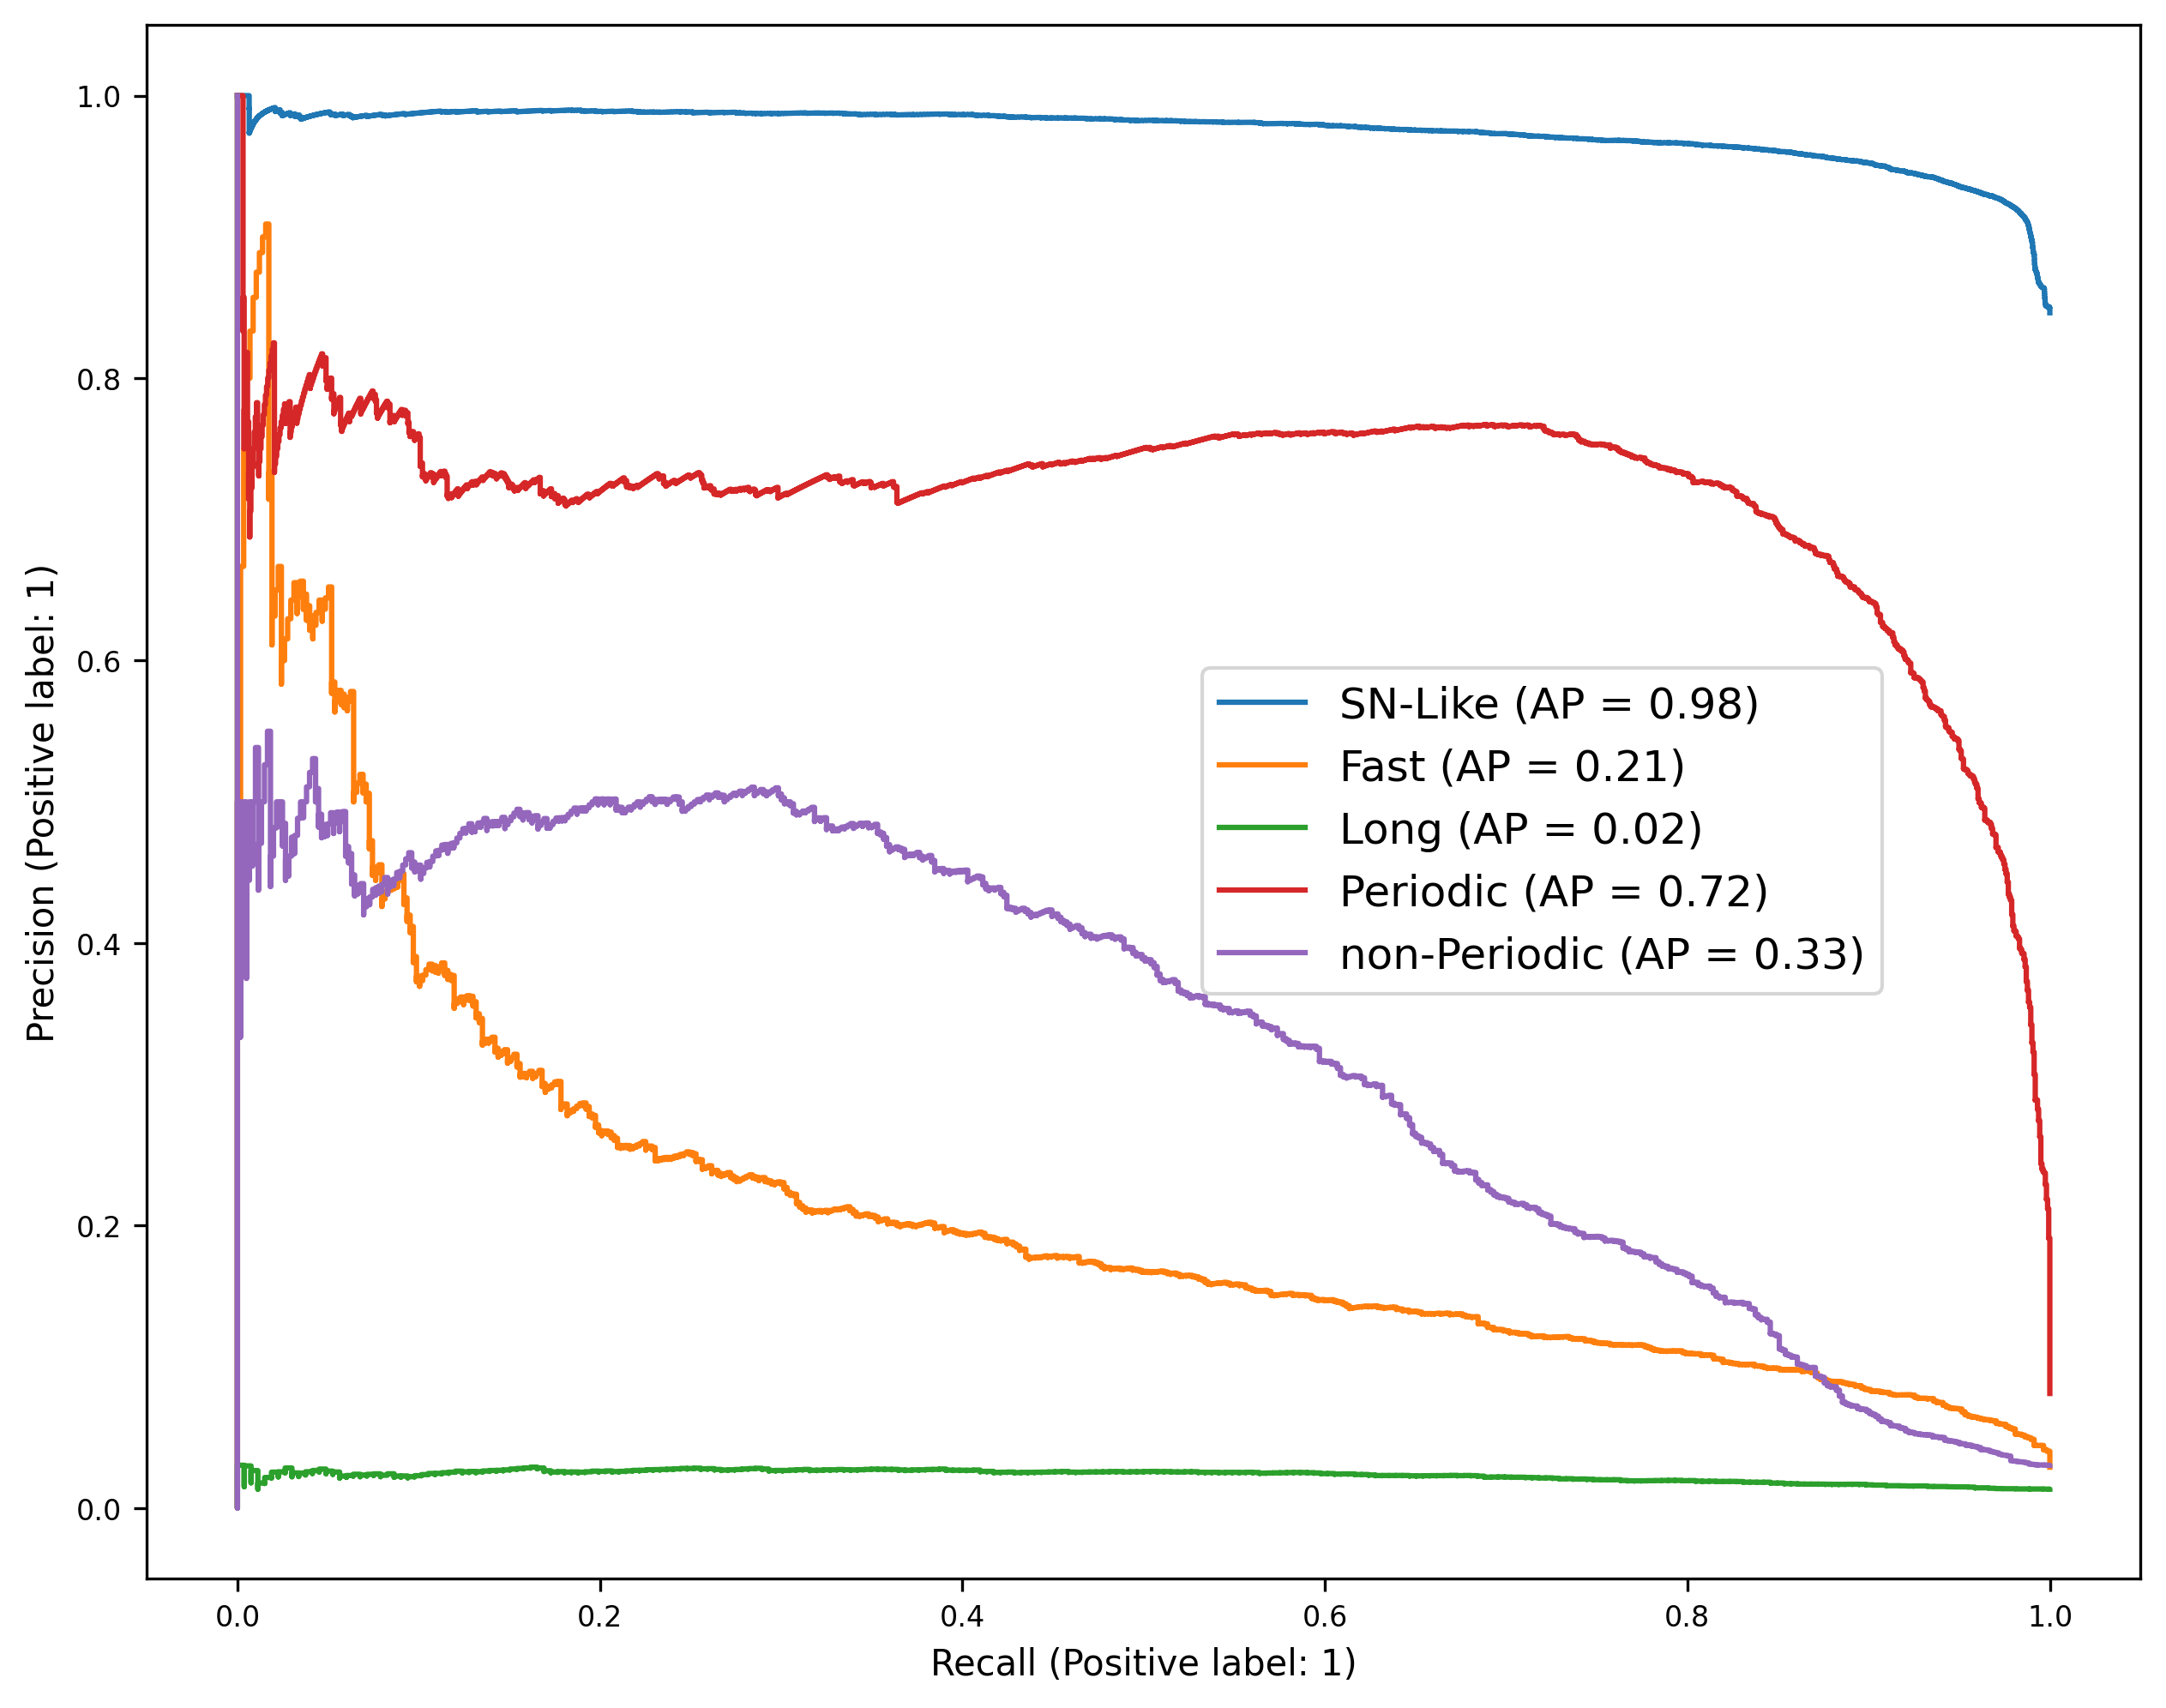
\includegraphics[width=0.5\textwidth]{figures/precision_5dias.png}}
    \hfill
    \subfigure[ROC curve for the dataset with a temporal advance of 5 days.]{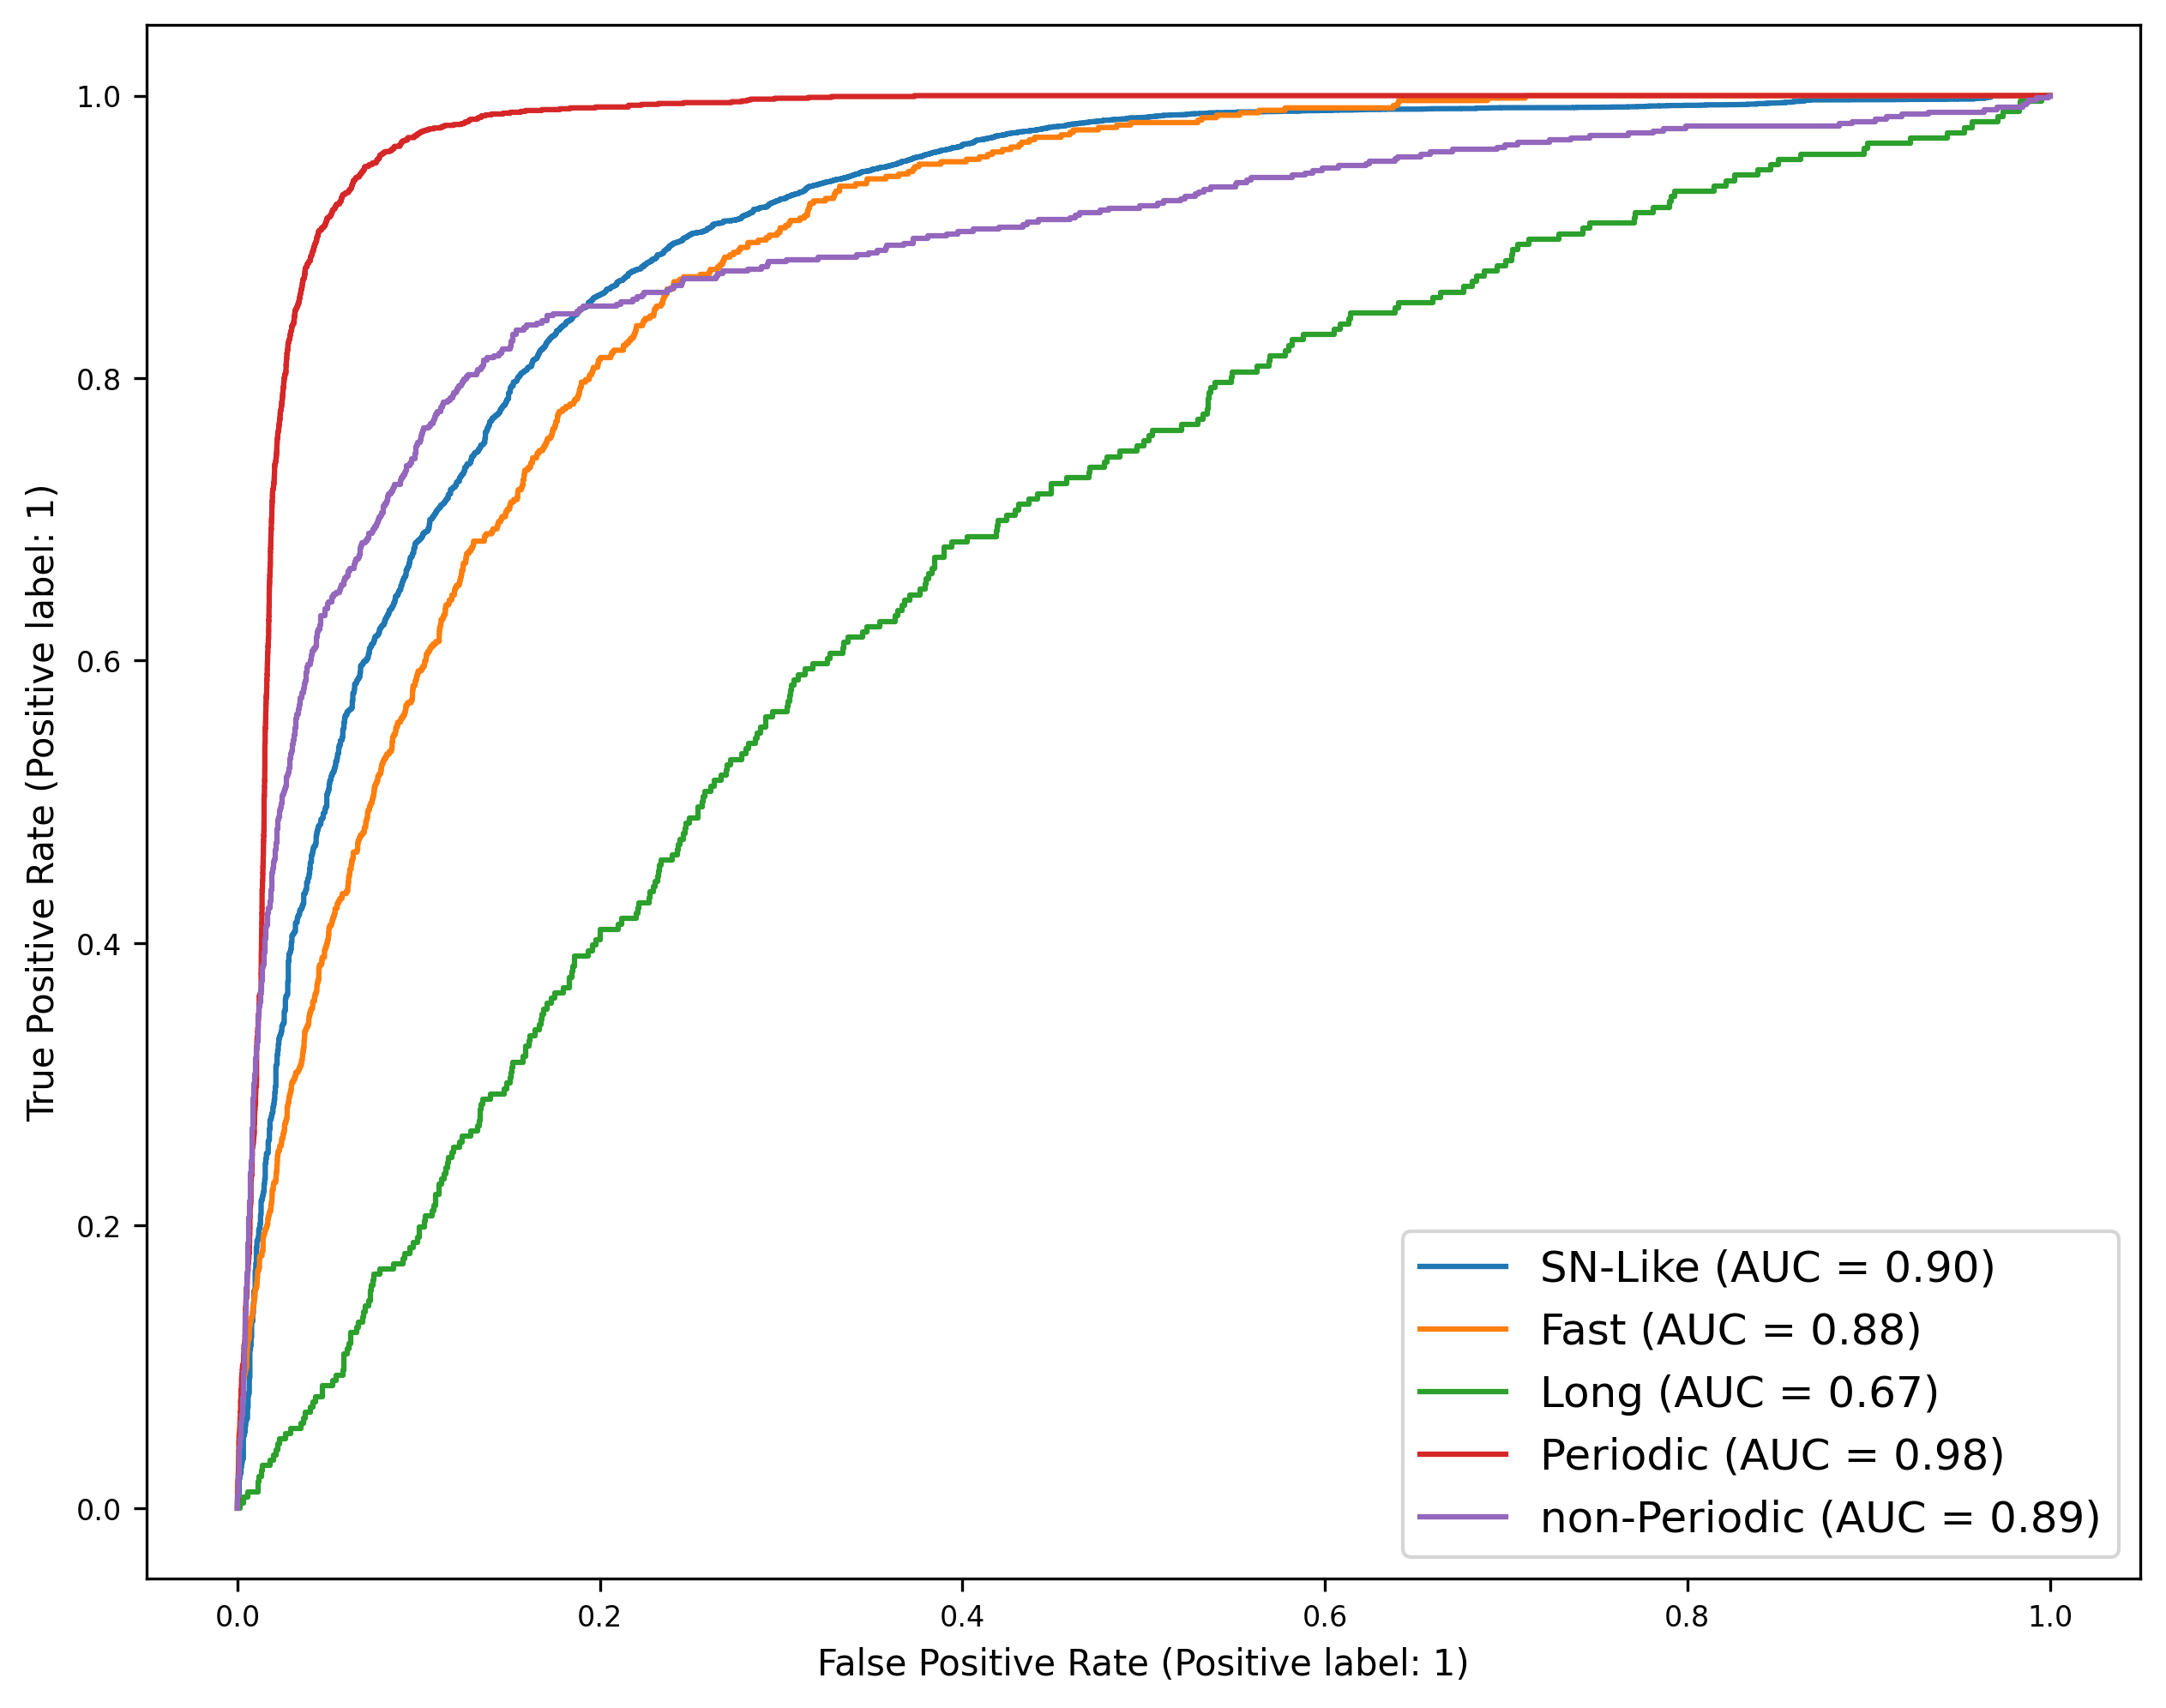
\includegraphics[width=0.5\textwidth]{figures/roc_5dias.png}}
    \caption{}
    \label{fig:roc e precision_5}
\end{figure}



\begin{figure}[!h]
    \centering
    \subfigure[Precision-Recall curve for the dataset with a temporal advance of 10 days.]{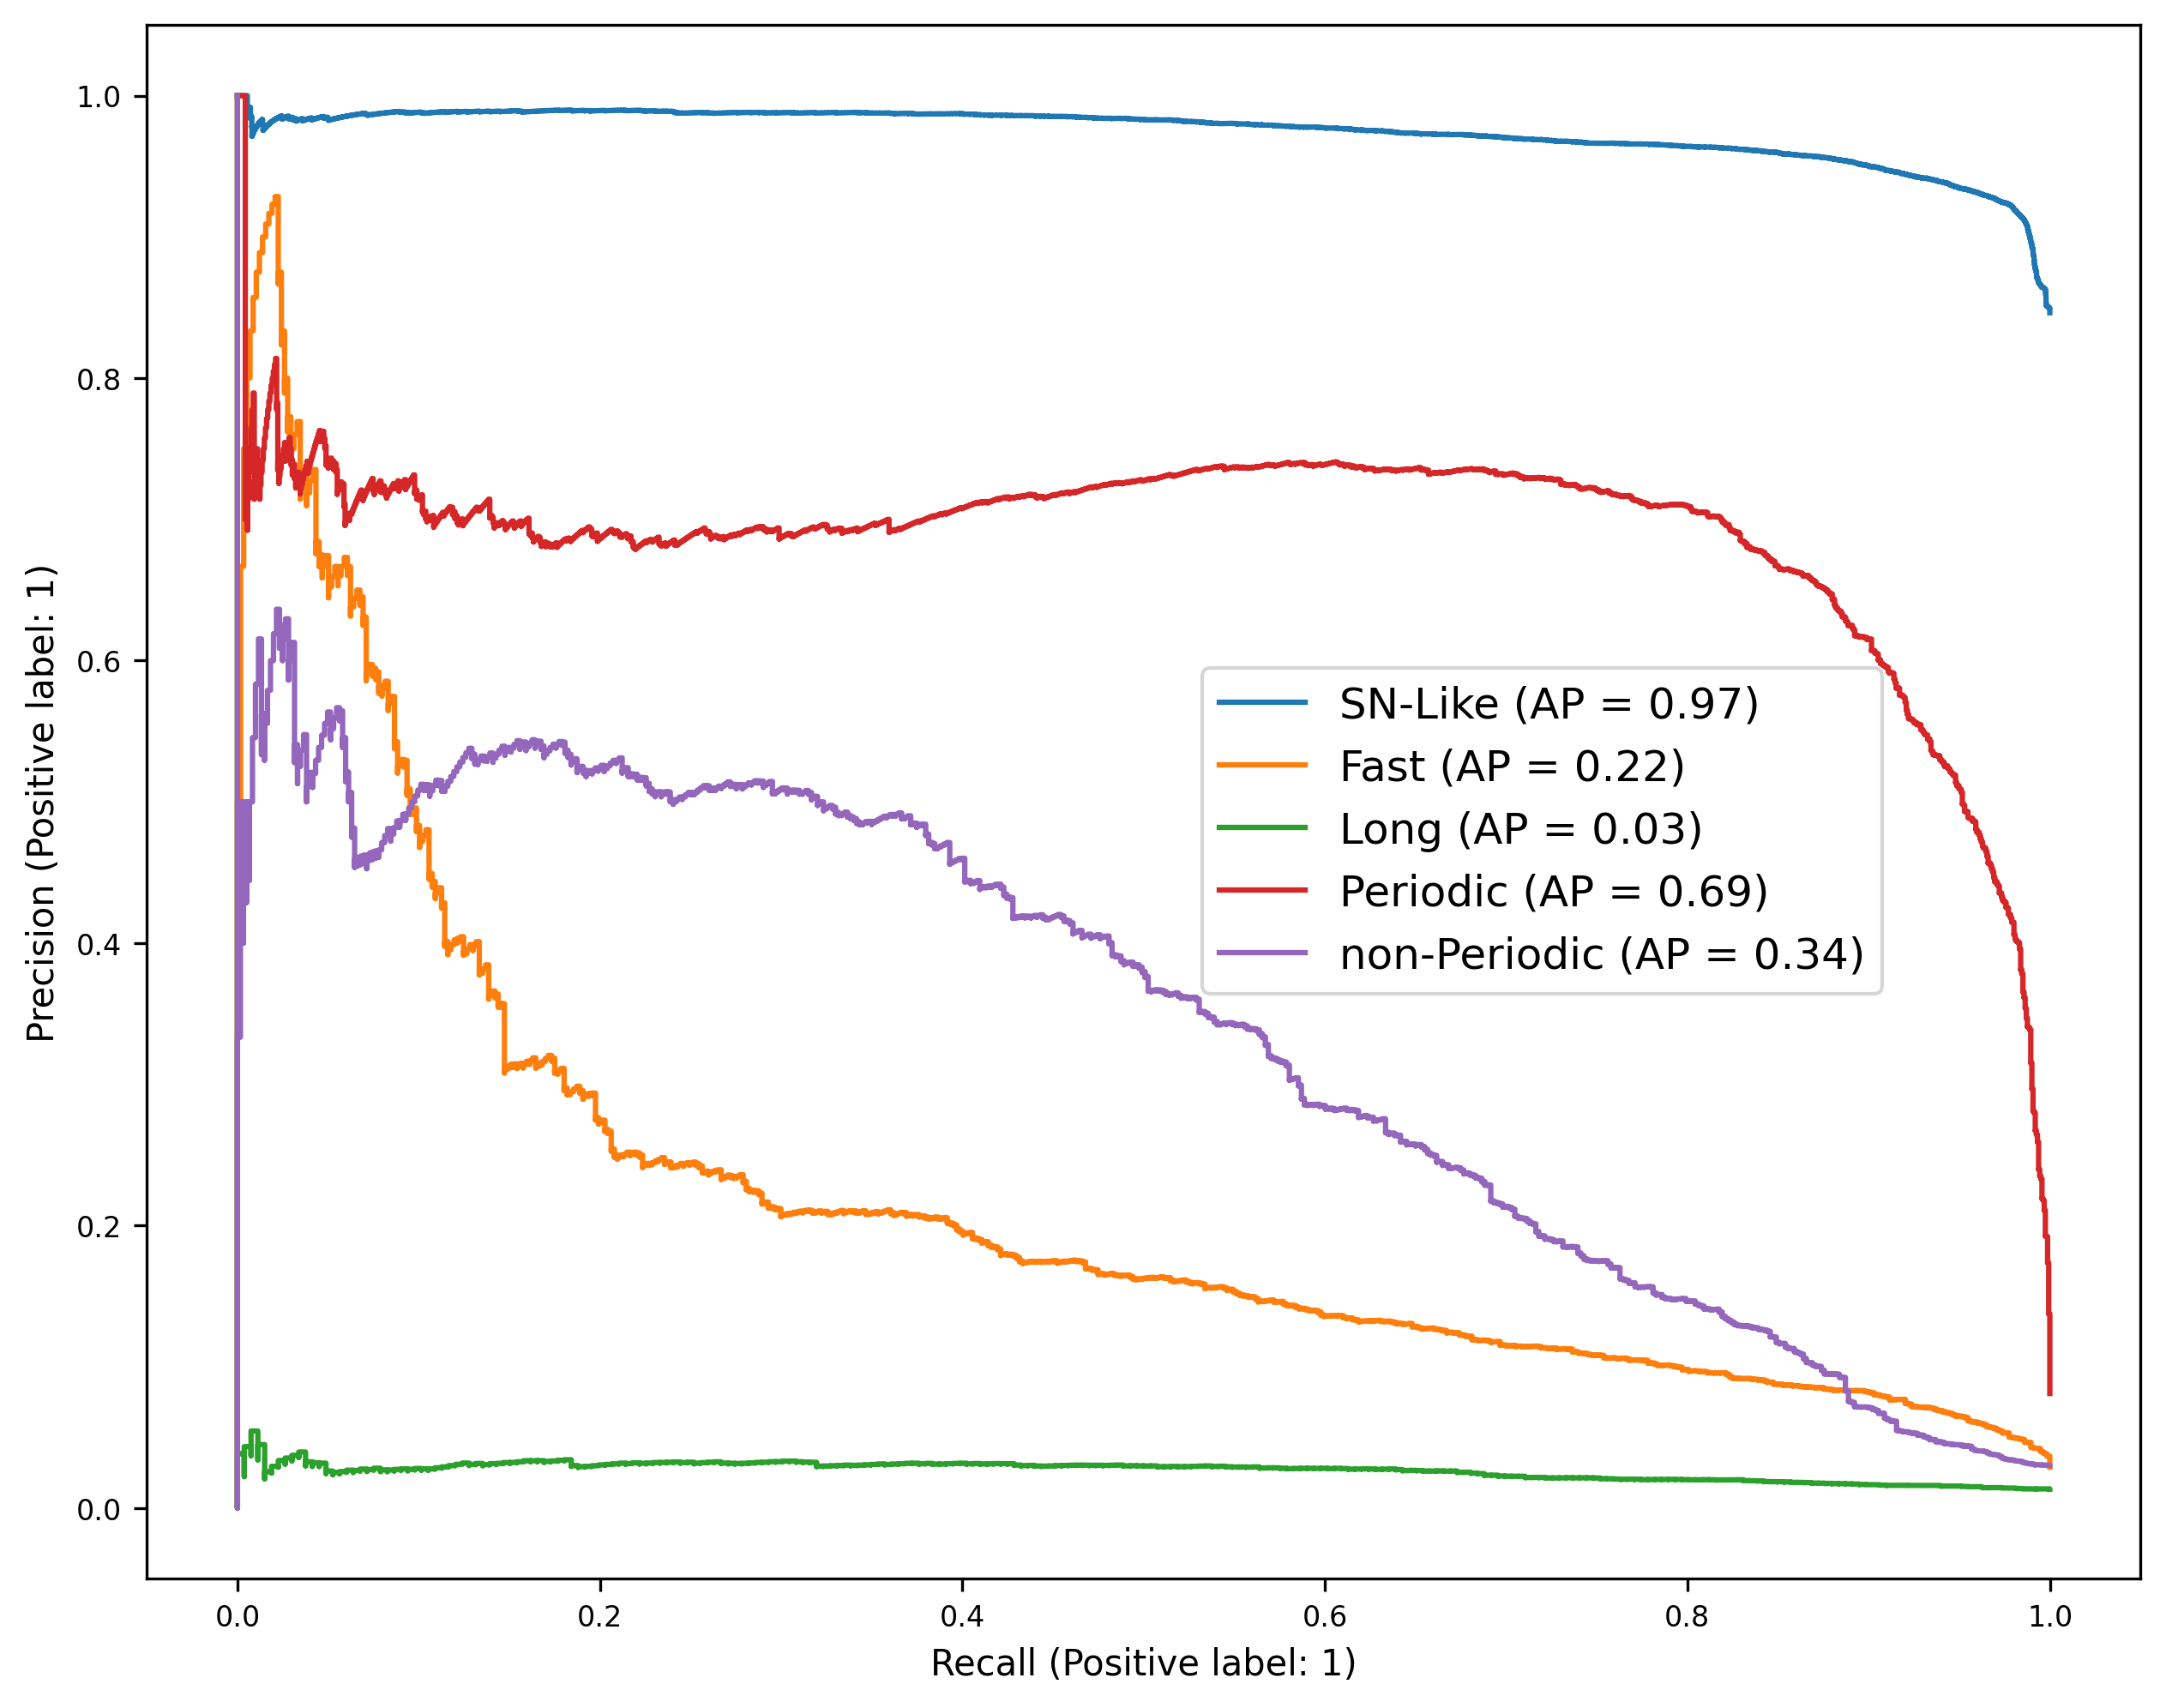
\includegraphics[width=0.5\textwidth]{figures/precision_10dias.png}}
    \hfill
    \subfigure[ROC curve for the dataset with a temporal advance of 10 days.]{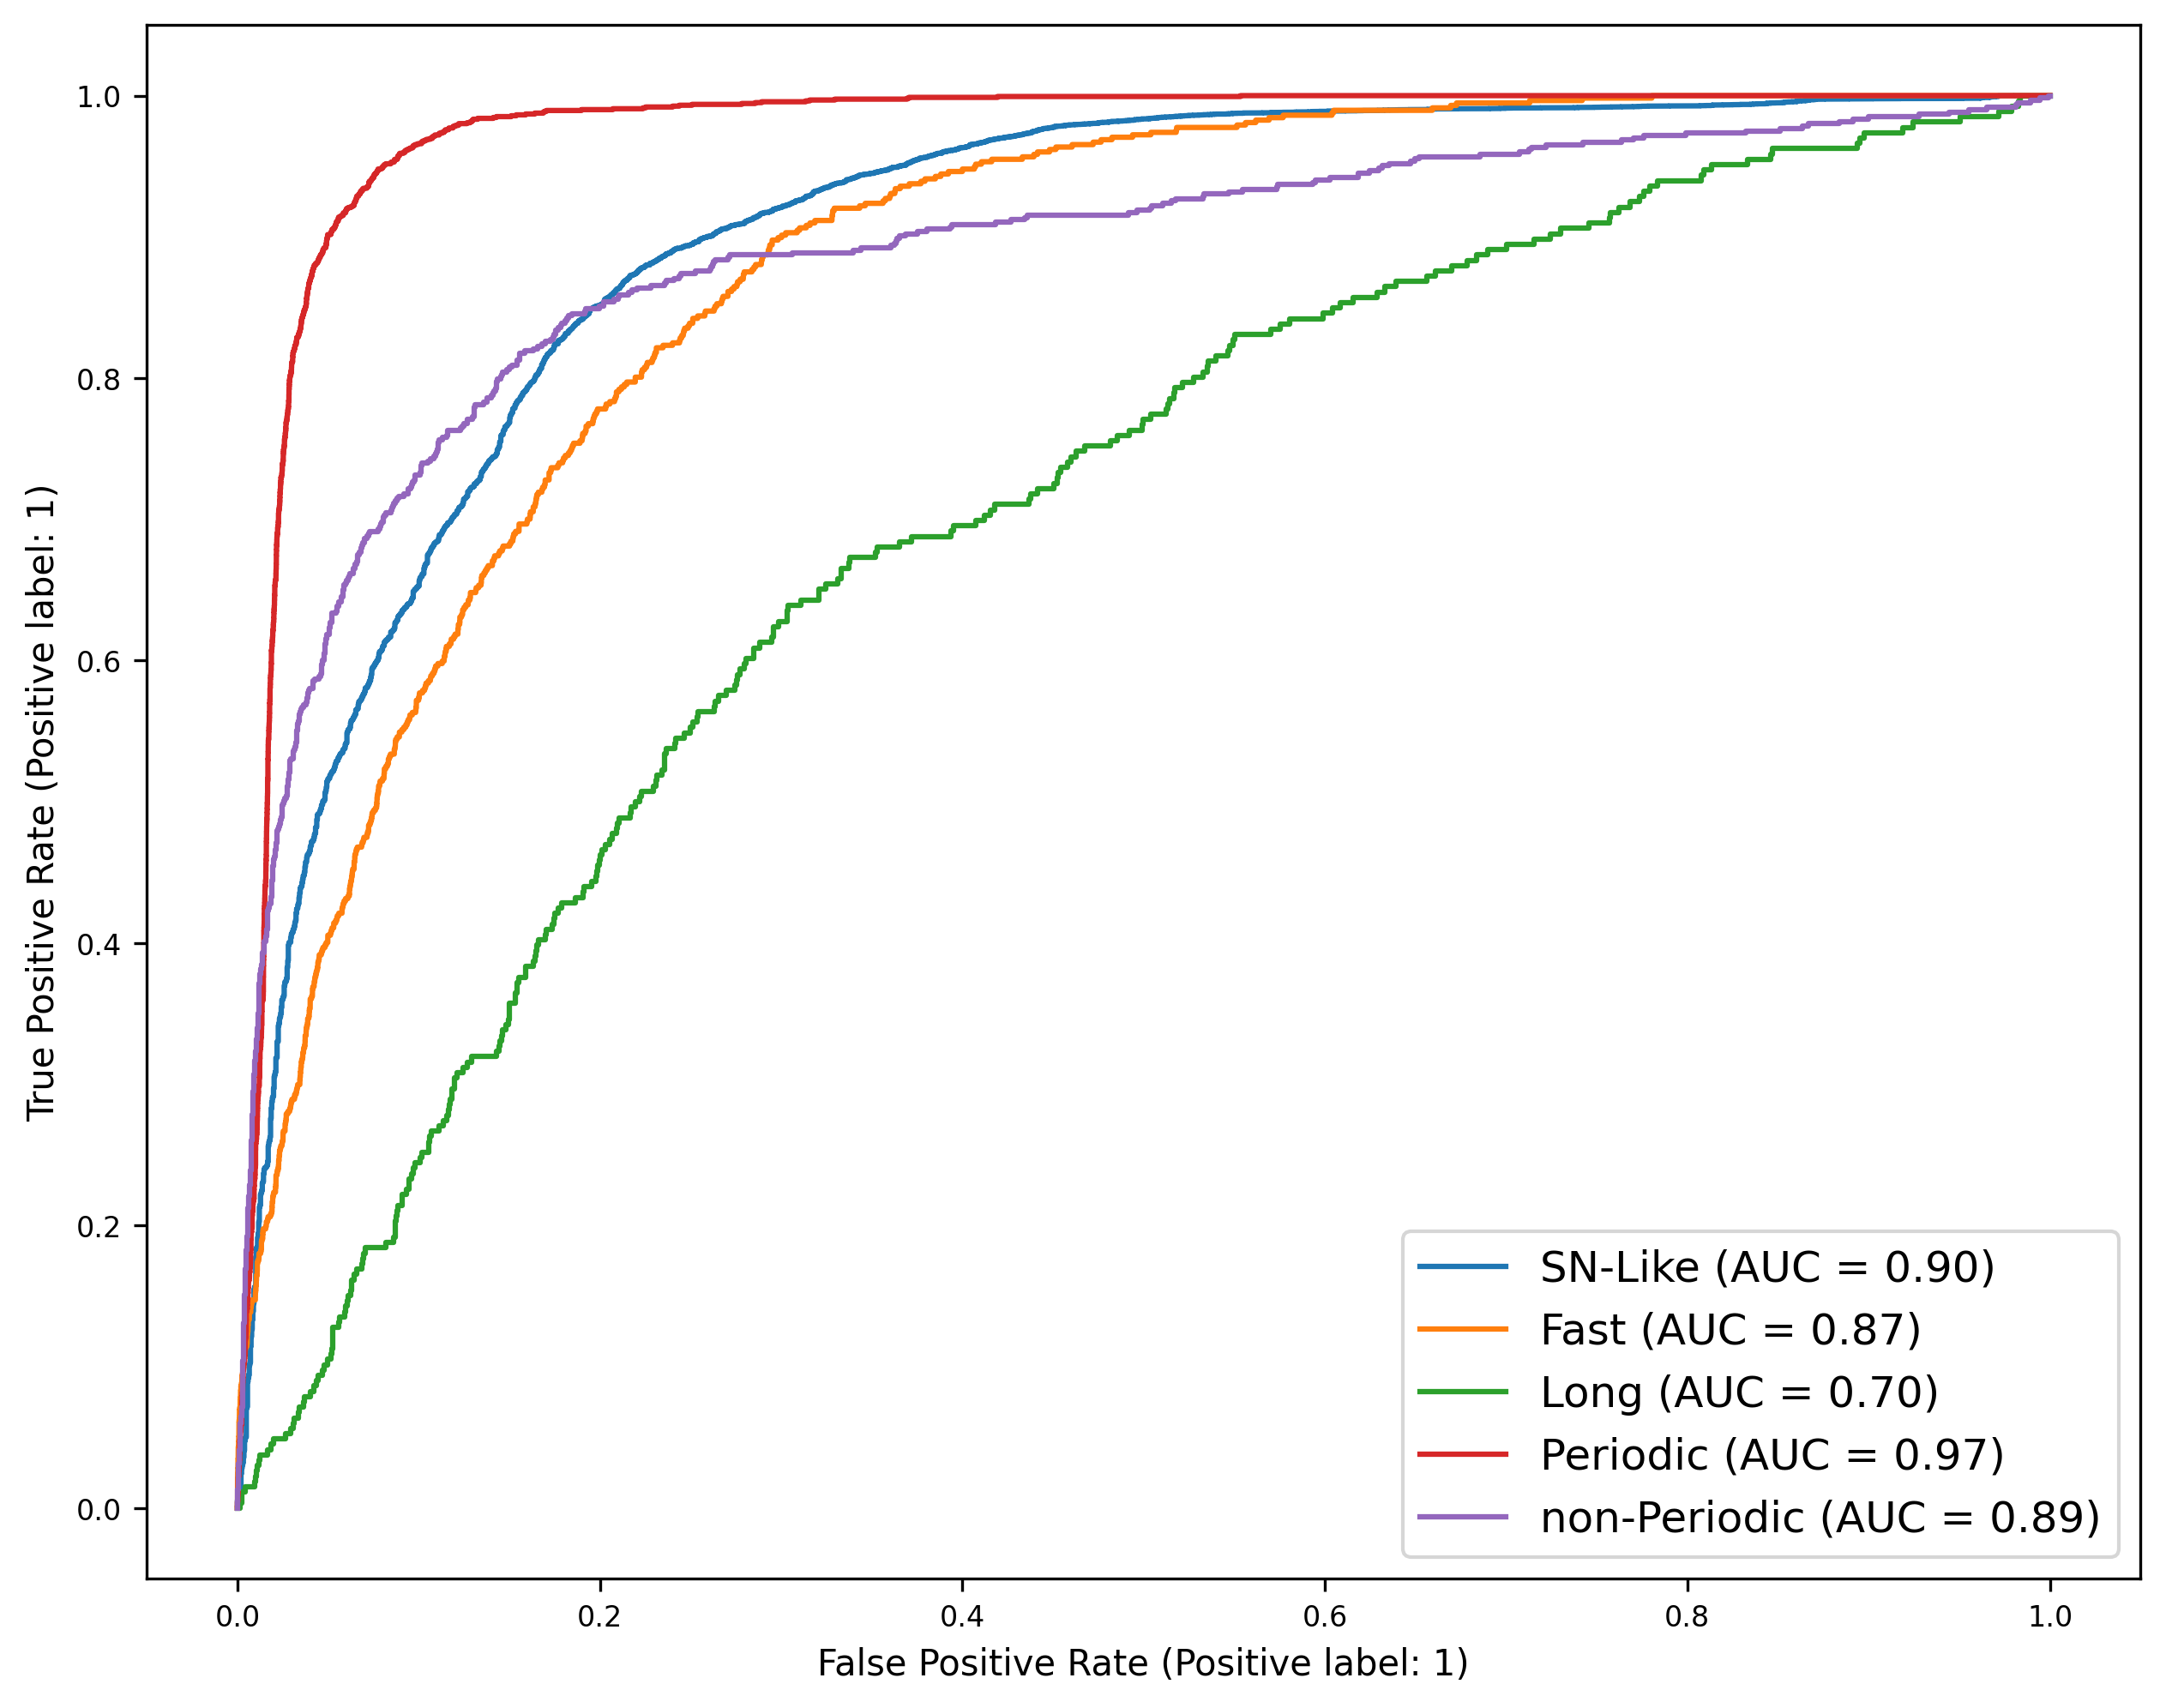
\includegraphics[width=0.5\textwidth]{figures/roc_10dias.png}}
    \caption{}
    \label{fig:roc e precision_10}
\end{figure}
\newpage

\begin{figure}[]
    \subfigure[Precision-Recall curve for the dataset with a temporal advance of 20 days.]{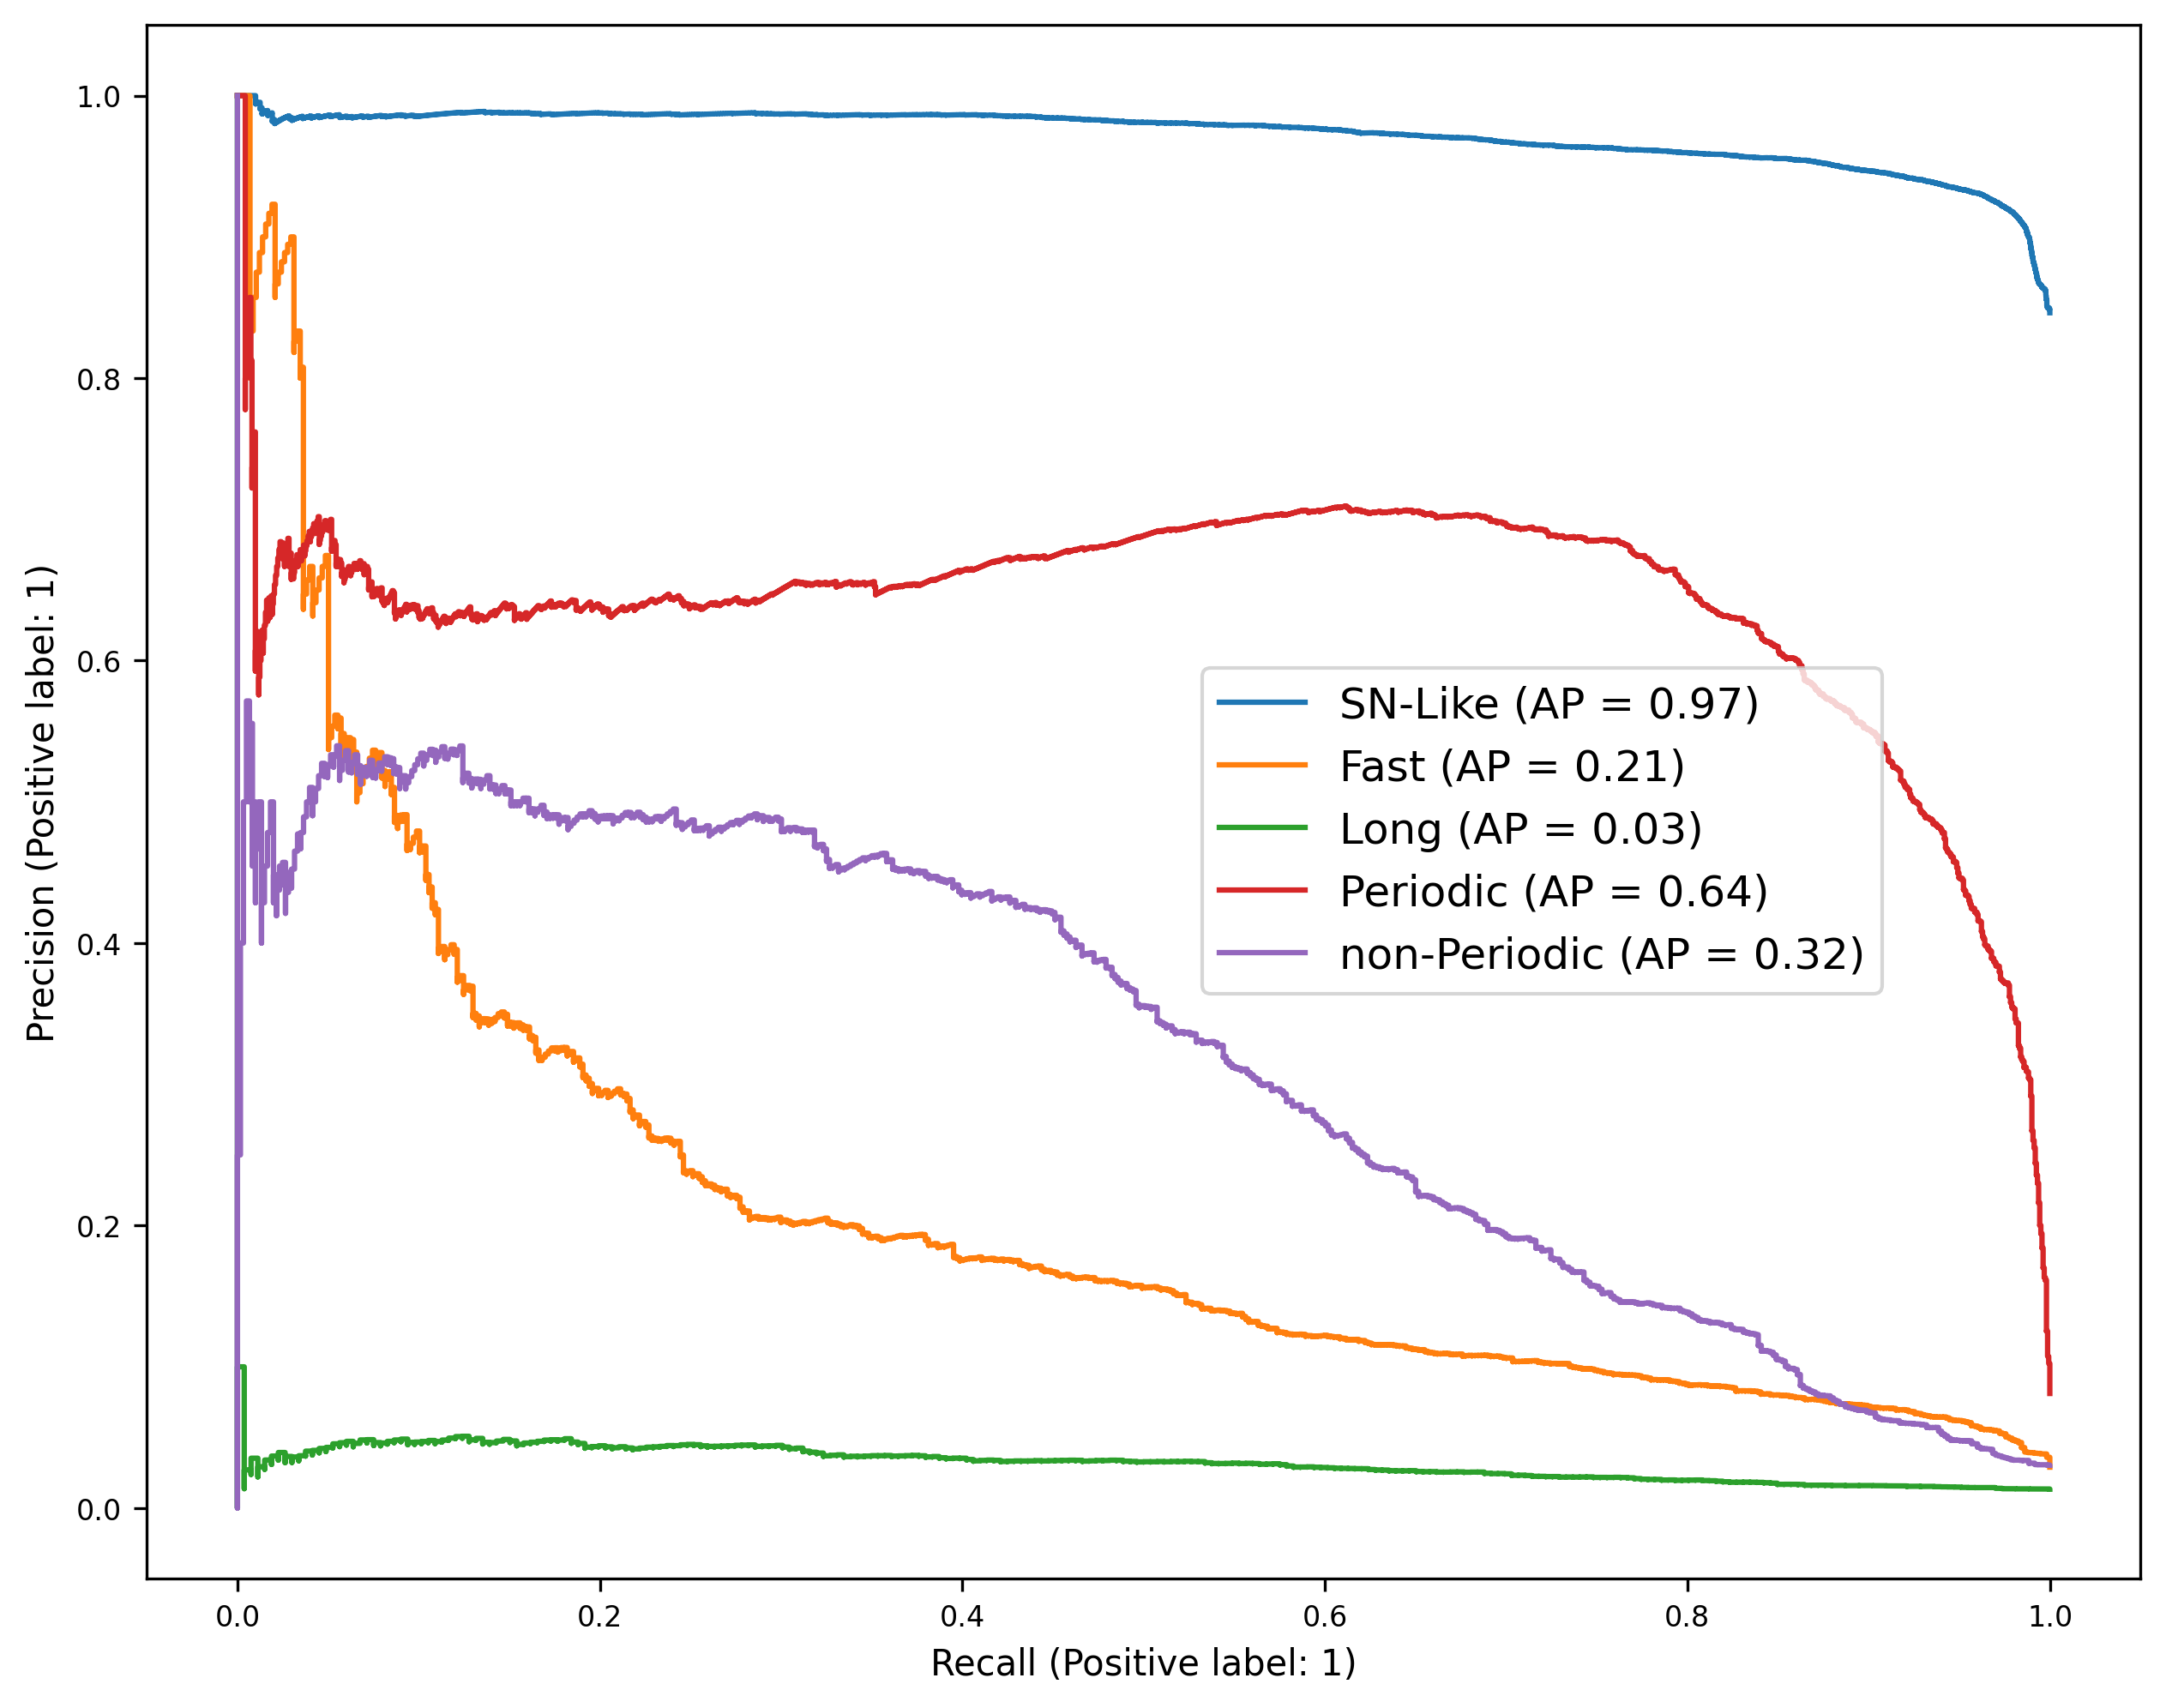
\includegraphics[width=0.5\textwidth]{figures/precision_20dias.png}}
    \hfill
    \subfigure[ROC curve for the dataset with a temporal advance of 20 days.]{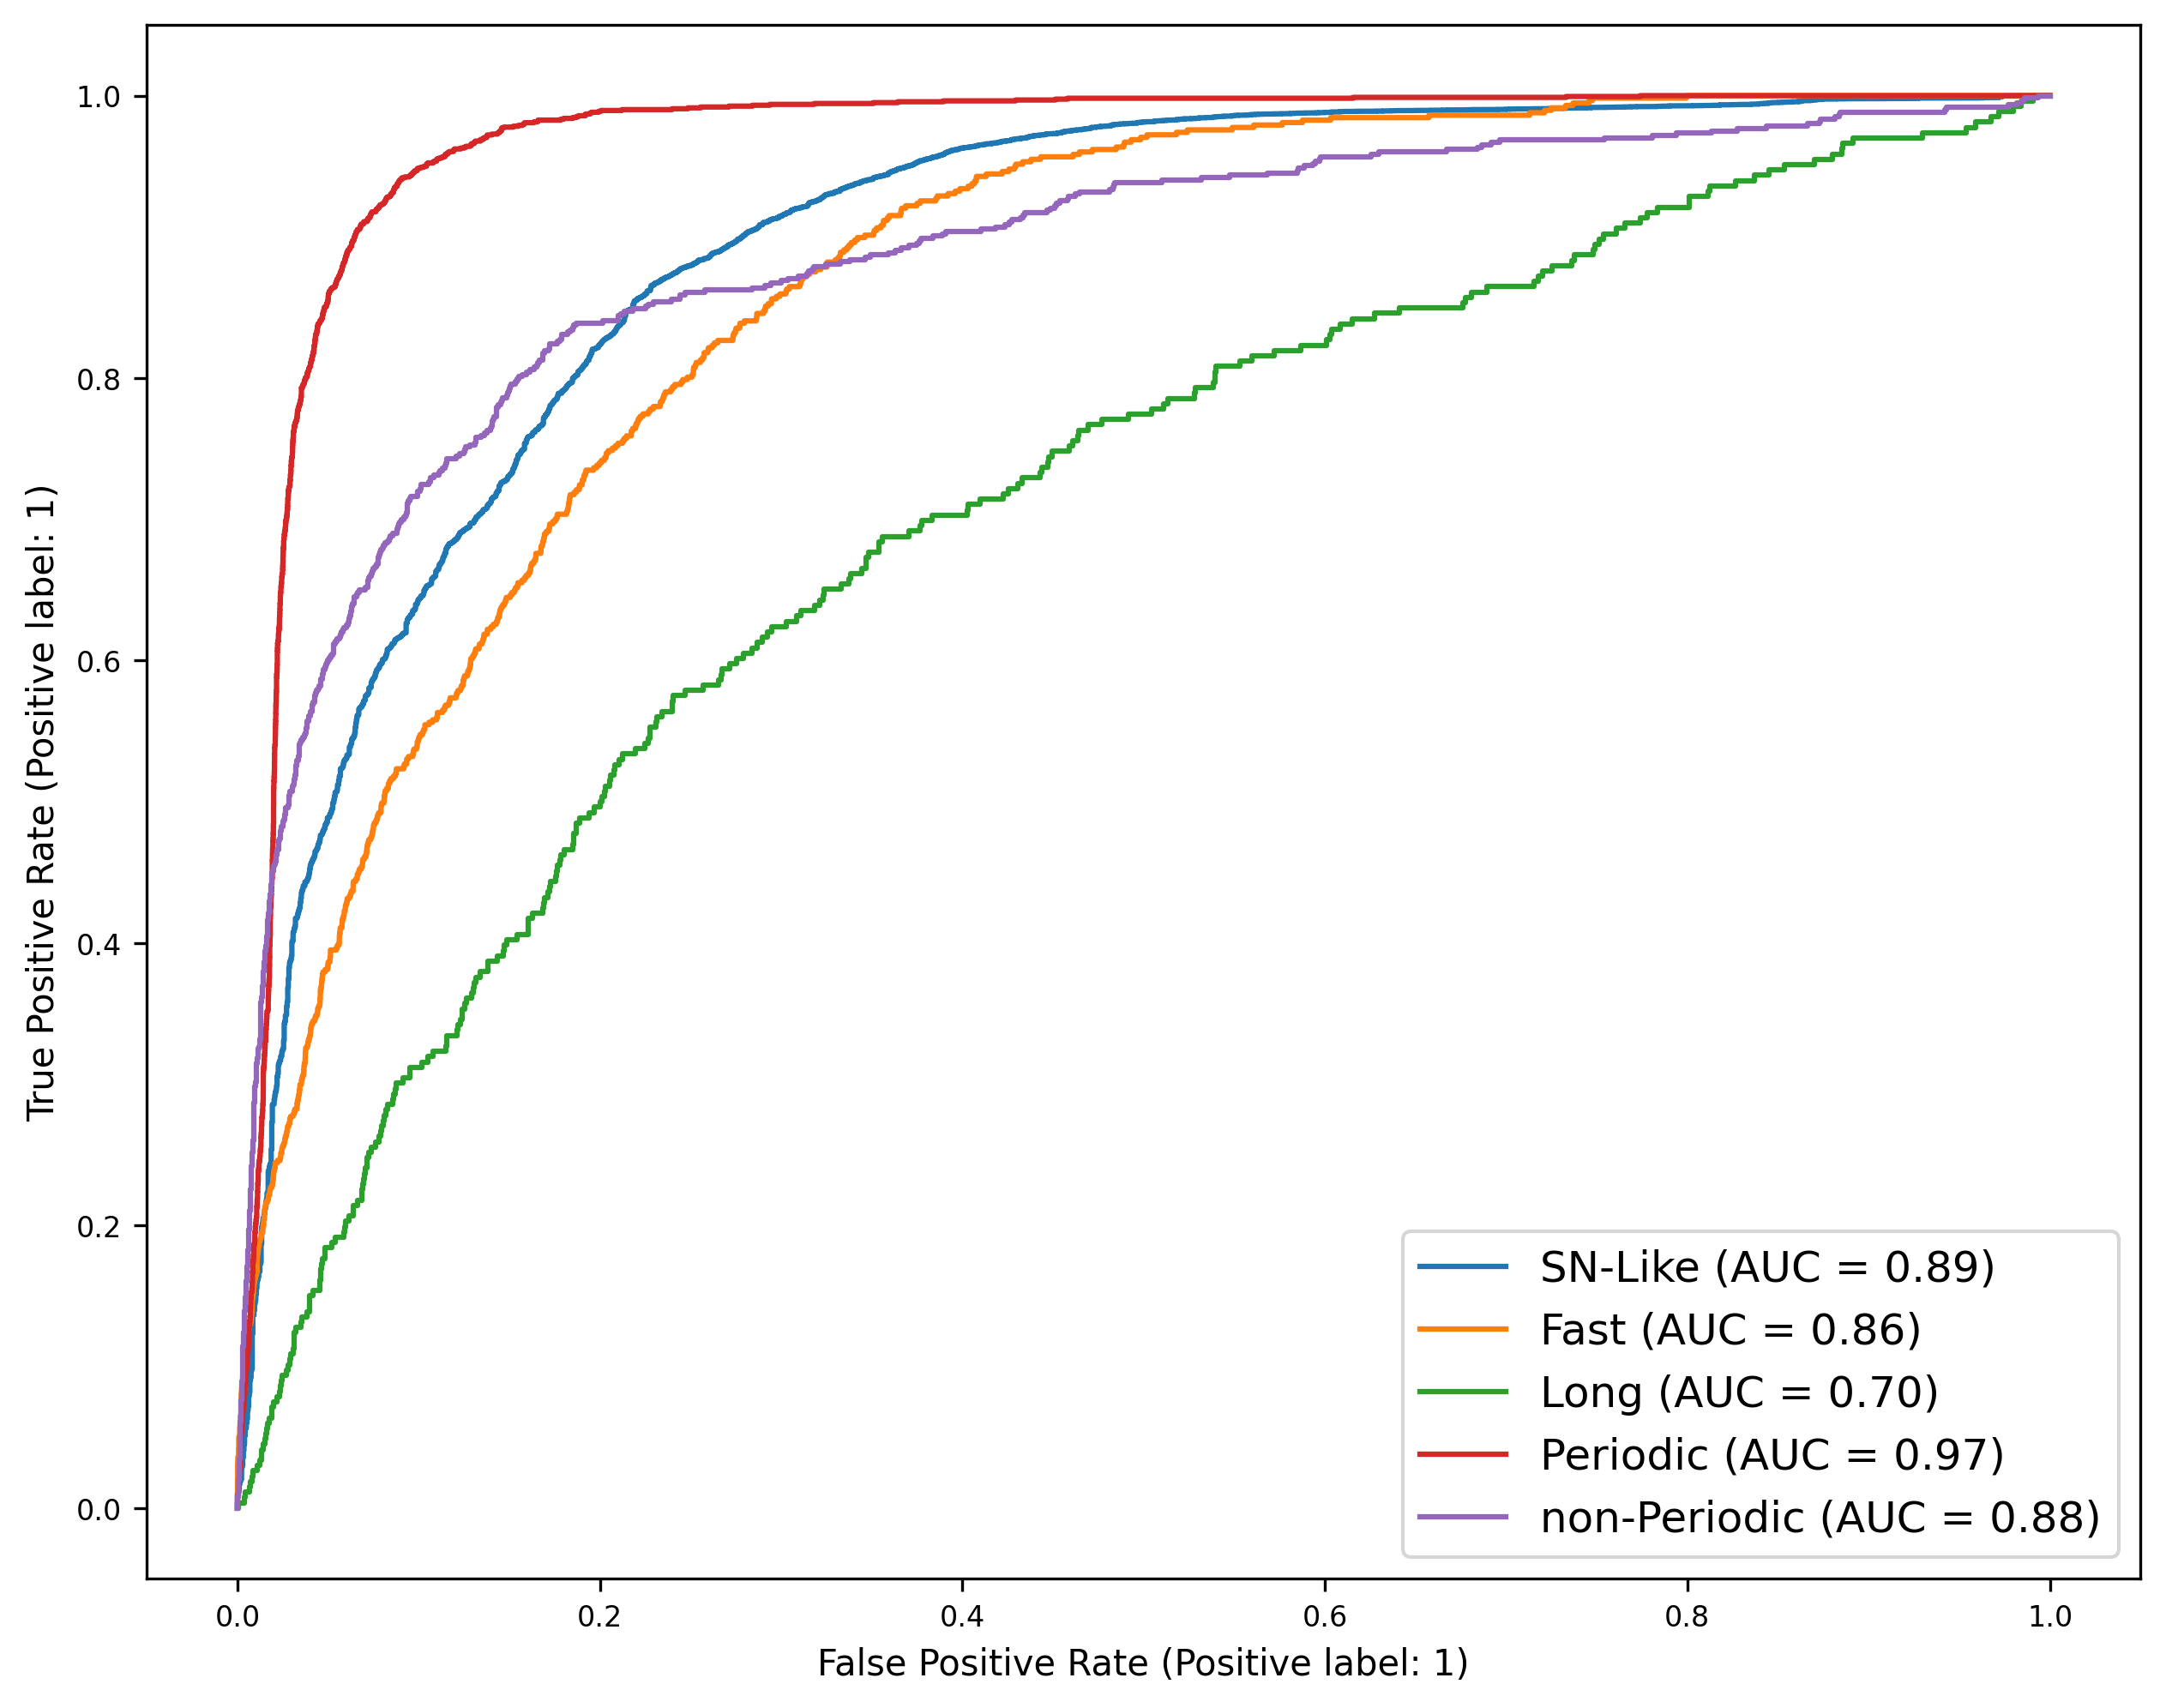
\includegraphics[width=0.5\textwidth]{figures/roc_20dias.png}}
    \caption{}
    \label{fig:roc e precision_20}
\end{figure}

\end{document}
%
